\subsection{可解李代数的嘉当子代数的共轭性}

设 g 是一个可解李代数。用 \(\mathcal{C}^{\infty}(\mathfrak{g})\) 表示 g 的下降中心列诸项的交（第一章，§1，第 5 节）。它是 g 的一个特征理想，并且是使 g/m 幂零的 g 的最小理想 m。由于 \(\mathcal{C}^{\infty}(\mathfrak{g}) \subset [\mathfrak{g}, \mathfrak{g}]\)，\(\mathcal{C}^{\infty}(\mathfrak{g})\) 是 g 的一个幂零理想（第一章，§5，第 3 节，定理 1 的推论 5）。由第 1 节的命题 1，诸 \(e^{ad x}\)（\(x \in \mathcal{C}^{\infty}(\mathfrak{g})\)）所成的集是 \(\operatorname{Aut}(\mathfrak{g})\) 的一个子群，包含在特殊自同构群内（第一章，§6，第 8 节，定义 6）。

定理 3. 设 \(\mathfrak{g}\) 是可解李代数，\(\mathfrak{h},\mathfrak{h}'\) 是 \(\mathfrak{g}\) 的嘉当子代数。则存在 \(x\in \mathcal{C}^{\infty}(\mathfrak{g})\) 使得 \(e^{\mathrm{ad}x}\mathfrak{h} = \mathfrak{h}'\)。

我们对 \(\dim \mathfrak{g}\) 作归纳，\(\mathfrak{g} = 0\) 的情形是平凡的。设 \(\mathfrak{n}\) 是 \(\mathfrak{g}\) 的一个极小非零交换理想。设 \(\varphi : \mathfrak{g} \to \mathfrak{g} / \mathfrak{n}\) 为典则态射。则有 \(\varphi(\mathcal{C}^{\infty} \mathfrak{g}) = \mathcal{C}^{\infty}(\mathfrak{g} / \mathfrak{n})\)（第一章，§1，第 5 节，命题 4）。由于 \(\varphi(\mathfrak{h})\) 与 \(\varphi(\mathfrak{h}')\) 都是 \(\mathfrak{g} / \mathfrak{n}\) 的嘉当子代数（§2，第 1 节，命题 4 的推论 2），由归纳假设，存在 \(x \in \mathcal{C}^{\infty}(\mathfrak{g})\) 使得 \(e^{\mathrm{ad} \varphi(x)}\varphi(\mathfrak{h}) = \varphi(\mathfrak{h}')\)。把 \(\mathfrak{h}\) 换成 \(e^{\mathrm{ad} x}\mathfrak{h}\)，即可假设 \(\varphi(\mathfrak{h}) = \varphi(\mathfrak{h}')\)，换言之，

\[
\mathfrak {h} + \mathfrak {n} = \mathfrak {h} ^ {\prime} + \mathfrak {n}.
\]

于是 \(\mathfrak{h}\) 与 \(\mathfrak{h}'\) 是 \(\mathfrak{h} + \mathfrak{n}\) 的嘉当子代数。若 \(\mathfrak{h} + \mathfrak{n} \neq \mathfrak{g}\)，则待证的断言由归纳假设得出。以下设 \(\mathfrak{h} + \mathfrak{n} = \mathfrak{h}' + \mathfrak{n} = \mathfrak{g}\)。

由 \(\mathfrak{n}\) 的极小性，有 \([\mathfrak{g},\mathfrak{n}] = \{0\}\) 或 \([\mathfrak{g},\mathfrak{n}] = \mathfrak{n}\)。若 \([\mathfrak{g},\mathfrak{n}] = \{0\}\)，则 \(\mathfrak{n} \subset \mathfrak{h}\) 且 \(\mathfrak{n} \subset \mathfrak{h}'\)（§2，第 1 节，命题 5），于是 \(\mathfrak{h} = \mathfrak{h} + \mathfrak{n} = \mathfrak{h}' + \mathfrak{n} = \mathfrak{h}'\)。剩下考虑 \([\mathfrak{g},\mathfrak{n}] = \mathfrak{n}\) 的情形，此时 \(\mathfrak{n} \subset \mathcal{C}^{\infty}(\mathfrak{g})\)。理想 \(\mathfrak{n}\) 是一个单 \(\mathfrak{g}\)-模；由于 \(\mathfrak{g} = \mathfrak{h} + \mathfrak{n}\)，且 \([\mathfrak{n},\mathfrak{n}] = \{0\}\)，可知 \(\mathfrak{n}\) 是一个单 \(\mathfrak{h}\)-模。若 \(\mathfrak{h} \cap \mathfrak{n} \neq \{0\}\)，则 \(\mathfrak{n} \subset \mathfrak{h}\)，于是 \(\mathfrak{g} = \mathfrak{h}\) 且 \(\mathfrak{h}' = \mathfrak{h}\)。现在设 \(\mathfrak{h} \cap \mathfrak{n} = \{0\}\)。则 \(\mathfrak{g} = \mathfrak{h} \oplus \mathfrak{n}\)，从而 \(\mathfrak{g} = \mathfrak{h}' \oplus \mathfrak{n}\)，因为 \(\mathfrak{h}\) 与 \(\mathfrak{h}'\) 有相同的维数。

对所有 \(x \in h\)，设 \(f(x)\) 是 n 中使 \(x - f(x) \in \mathfrak{h}'\) 的唯一元素；若 \(x, y \in h\)，

\[
[ x, y ] - [ x, f (y) ] - [ f (x), y ] = [ x - f (x), y - f (y) ] \in \mathfrak {h} ^ {\prime},
\]

于是 \(f([x,y]) = [x,f(y)] + [f(x),y]\)。由 §1 第 3 节命题 9 的推论，存在 \(a \in \mathfrak{n}\) 使得 \(f(x) = [x,a]\) 对所有 \(x \in \mathfrak{h}\) 成立。我们有 \((\operatorname{ad}a)^2(\mathfrak{g}) \subset (\operatorname{ad}a)(\mathfrak{n}) = 0\)，故对所有 \(x \in \mathfrak{h}\)，

\[
e ^ {\operatorname{ad} a} x = x + [ a, x ] = x - f (x).
\]

这样就有 \(e^{\mathrm{ad}a}(\mathfrak{h}) = \mathfrak{h}'\)。由于 \(a \in \mathcal{C}^{\infty}(\mathfrak{g})\)，证明完毕。

引理 3. 设 g 是李代数，r 是其根基，\(\varphi\) 是 g 到 g/r 的典则同态，v 是 g/r 的一个初等自同构。则存在 g 的初等自同构 u 使得 \(\varphi \circ u = v \circ \varphi\)。

我们可以假设 \(v\) 形如 \(e^{\mathrm{ad}b}\)，其中 \(b \in \mathfrak{g} / \mathfrak{r}\) 且 \(\mathrm{ad}b\) 幂零。设 \(\mathfrak{s}\) 是 \(\mathfrak{g}\) 的一个 Levi 子代数（第一章，§6，第 8 节，定义 7），并设 \(a\) 是 \(\mathfrak{s}\) 中使 \(\varphi(a) = b\) 的元素。由于 \(\mathrm{ad}_{\mathfrak{s}}a\) 幂零，\(\mathrm{ad}_{\mathfrak{g}}a\) 幂零（第一章，§6，第 3 节，命题 3 的推论），且 \(u = e^{\mathrm{ad}_{\mathfrak{g}}a}\) 是 \(\mathfrak{g}\) 的一个初等自同构，满足 \(\varphi \circ u = v \circ \varphi\)。

命题 5. 设 g 是李代数，r 是其根基，h 与 h' 是 g 的嘉当子代数，\(\varphi\) 是 g 到 g/r 的典则同态。下列条件等价：

\begin{enumerate}
\def\labelenumi{(\roman{enumi})}
\item
  \(\mathfrak{h}\) 与 \(\mathfrak{h}'\) 经 \(\mathfrak{g}\) 的一个初等自同构共轭；
\item
  \(\varphi (\mathfrak{h})\) 与 \(\varphi (\mathfrak{h}^{\prime})\) 经 \(\mathfrak{g} / \mathfrak{r}\) 的一个初等自同构共轭。
\item
  \(\Longrightarrow\) (ii)：这是显然的。
\item
  \(\Longrightarrow\) (i)：假设条件 (ii) 成立，证明 (i)。由引理 3，可化为 \(\varphi(\mathfrak{h}) = \varphi(\mathfrak{h}')\) 的情形。置 \(\mathfrak{k} = \mathfrak{h} + \mathfrak{r} = \mathfrak{h}' + \mathfrak{r}\)，它是 \(\mathfrak{g}\) 的一个可解子代数。于是 \(\mathfrak{h}\) 与 \(\mathfrak{h}'\) 是 \(\mathfrak{k}\) 的嘉当子代数，故存在 \(x \in \mathcal{C}^{\infty}(\mathfrak{k})\) 使得 \(e^{\mathrm{ad}_{\mathfrak{k}}x}\mathfrak{h} = \mathfrak{h}'\)（定理 3）。由于 \(\mathfrak{k}/\mathfrak{r}\) 幂零，\(\mathcal{C}^{\infty}(\mathfrak{k}) \subset \mathfrak{r}\)；另一方面，\(\mathcal{C}^{\infty}(\mathfrak{k}) \subset [\mathfrak{k},\mathfrak{k}] \subset [\mathfrak{g},\mathfrak{g}]\)，故 \(x \in \mathfrak{r} \cap [\mathfrak{g},\mathfrak{g}]\)；由第一章 §5 第 3 节定理 1，\(\mathrm{ad}_{\mathfrak{g}}x\) 幂零，从而 \(e^{\mathrm{ad}_{\mathfrak{g}}x}\) 是 \(\mathfrak{g}\) 的一个把 \(\mathfrak{h}\) 变换为 \(\mathfrak{h}'\) 的初等自同构。
\end{enumerate}

\subsection{李群情形}

命题 6. 设 k 是 R、C 或特征为 0 的非离散完备超度量域。设 G 是 k 上的一个有限维李群，e 是其单位元，g 是其李代数，h 是 g 的一个嘉当子代数，\(h_{r}\) 是 g 中属于 h 的正则元所成的集。

\begin{enumerate}
\def\labelenumi{(\roman{enumi})}
\item
  设 \(\mathfrak{s}\) 是 \(\mathfrak{h}\) 在 \(\mathfrak{g}\) 中的一个向量空间补，\(\mathfrak{s}_0\) 是 \(\mathfrak{s}\) 中 0 的一个在其上定义了指数映射的邻域，且 \(h_0 \in \mathfrak{h}_r\)。映射 \((s, h) \mapsto \mathrm{F}(s, h) = (\exp \operatorname{ad} s).h\)（从 \(\mathfrak{s}_0 \times \mathfrak{h}\) 到 \(\mathfrak{g}\)）在 \((0, h_0)\) 处是平展的。
\item
  映射 \((g,h)\mapsto \mathrm{F}'(g,h) = (\operatorname {Ad}g).h\)（从 \(\mathbf{G}\times \mathfrak{h}_r\) 到 \(\mathfrak{g}\)）是一个浸没。特别地，其像 \(\Omega\) 是开集。对所有 \(x\in \Omega\)，\(\mathfrak{g}^0 (x)\) 是 \(\mathfrak{g}\) 的一个与 \(\mathfrak{h}\) 在 \(\operatorname {Ad}(\mathrm{G})\) 下共轭的嘉当子代数
\item
  设 \(h_0 \in \mathfrak{h}_r\)。对任意邻域 \(\mathrm{U}\)（\(e\) 在 \(\mathrm{G}\) 中的一个邻域），集合 \(\bigcup_{a \in \mathrm{U}} (\mathrm{Ad}a)(\mathfrak{h}_r)\) 是 \(h_0\) 在 \(\mathfrak{g}\) 中的一个邻域。
\end{enumerate}

设 \(h_0\) 与 \(\mathfrak{s}\) 如 (i) 中所述。设 \(\mathrm{T}\) 是 \(\mathrm{F}\) 在 \((0, h_0)\) 处的切线性映射。于是 \(\mathrm{F}(0, h) = h\) 对所有 \(h \in \mathfrak{h}\) 成立，故 \(\mathrm{T}(0, h) = h\) 对所有 \(h \in \mathfrak{h}\) 成立。另一方面，当 \(\mathfrak{s}_0\) 充分小时，映射 \(s \mapsto \exp s\)（从 \(\mathfrak{s}_0\) 到 \(\operatorname{End}(\mathfrak{g})\)）在 0 处的切线性映射就是映射 \(s \mapsto \operatorname{ad}s\)（从 \(\mathfrak{s}\) 到 \(\operatorname{End}(\mathfrak{g})\)）。于是 \(\mathrm{T}(s, 0) = [s, h_0]\) 对所有 \(s \in \mathfrak{s}\) 成立。而从 \(\mathfrak{g}/\mathfrak{h}\) 到 \(\mathfrak{g}/\mathfrak{h}\) 的、由 \(\operatorname{ad}h_0\) 过渡到商所诱导的映射是双射的。由此推出 \(\mathrm{T}\) 是双射，从而得出 (i)。由于 \(\exp s = \operatorname{Ad}\exp s\) 对所有充分接近 0 的 \(s \in \mathfrak{s}\) 成立，(iii) 与 (ii) 的第一个断言随之成立。每个 \(x \in \Omega\) 都形如 \((\operatorname{Ad}a)(h)\)，其中 \(a \in G\)，\(h \in \mathfrak{h}_r\)，于是 \(\mathfrak{g}^0(x) = (\operatorname{Ad}a)(\mathfrak{g}^0(h)) = (\operatorname{Ad}a)(\mathfrak{h})\) 是 \(\mathfrak{g}\) 的一个与 \(\mathfrak{h}\) 在 \(\operatorname{Ad}(G)\) 下共轭的子代数。

\section{李群的正则元}

在本 § 的第 1、2、3 节中，我们假设 k 是 R、C 或特征为 0 的非离散完备超度量域。我们用 G 表示 k 上的一个有限维李群，用 g 表示它的李代数，并用 e 表示它的单位元。若 \(a \in G\)，我们用 \(\mathfrak{g}^{1}(a)\) 表示 \(\operatorname{Ad}(a) - 1\) 的幂零空间，换言之即空间 \(\mathfrak{g}^{1}(\operatorname{Ad}(a))\)（参见 §1，第 1 节）。

\subsection{线性表示的正则元}

引理 1. 设 M 是 k 上的一个解析流形，\(a = (a_{0}, \ldots, a_{n-1}, a_{n} = 1)\) 是 M 上的一个解析函数序列。对所有 \(x \in M\)，设 \(r_{a}(x)\) 是那些 \(i \in [0, n]\)（它们满足 \(a_{j}(x) = 0\)，其中 j \textless{} i）的上确界，并设 \(r_{a}^{0}(x)\) 是那些 \(i \in [0, n]\)（对它们，\(a_{j}\) 在 x 的一个邻域上为零，其中 j \textless{} i）的上确界。

\begin{enumerate}
\def\labelenumi{(\roman{enumi})}
\item
  函数 \(r_a\) 是上半连续的。
\item
  对所有 \(x \in \mathrm{M}\)，\(r_a^0(x) = \liminf_{y \to x} r_a(y)\)。
\item
  函数 \(r_a^0\) 是局部常值的。
\item
  点 \(x \in M\)（满足 \(r_{a}^{0}(x) = r_{a}(x)\)）所成的集，就是在 \(r_{a}\) 于其一个邻域上取常值的 M 的点所成的集。这是 M 的一个稠密开子集。若 k = C 且 M 有限维并连通，则它还是开且连通的。
\item
  若 \(r_a(x) = i\)，则 \(a_i(x) \neq 0\)，且对所有 \(y\)（\(x\) 的一个邻域中的点），有 \(a_i(y) \neq 0\)，从而 \(r_a(y) \leq i\)。
\item
  若 \(r_{a}^{0}(x) = i\)，则函数 \(a_{0}, \ldots, a_{i-1}\) 在 x 的一个邻域上为零，且对该邻域中的任何 y，\(r_{a}(y) \geq i\)。因而 \(\liminf_{y \to x} r_{a}(y) \geq i\)。x 的每个邻域都含一点 y，使 \(a_{i}(y) \neq 0\)，从而 \(r_{a}(y) \leq i\)。于是 \(\liminf_{y \to x} r_{a}(y) = i\)。
\item
  设 \(i = r_a^0 (x)\)，并设 \(V\) 是 \(x\) 的一个邻域，使得 \(a_{j}(y) = 0\) 对所有 \(y\in V\) 和所有 \(j < i\) 成立。则 \(x\in M - Z\)，其中 \(Z\) 表示 \(M\) 中在其一个邻域上函数 \(a_{i}\) 为零的点所成的集。由于 \(Z\) 在 \(M\) 中是闭的（《微分与解析流形·结果》，5.3.5），\(V\cap (M - Z)\) 是 \(x\) 的一个邻域。对此邻域中的每一点 \(y\)，有 \(r_a^0 (y) = i\)。
\item
  函数 \(r_{a}-r_{a}^{0}\) 是上半连续的，且它在任一点的值都 \(\geq0\)。若 \(r_{a}(x)=r_{a}^{0}(x)\)，则 \(r_{a}-r_{a}^{0}\) 在 x 的一个邻域上为零，由 (iii) 这表明 \(r_{a}\) 在 x 的一个邻域上为常数。反之，若 \(r_{a}\) 在 x 的一个邻域上为常数，则由 (ii) 有 \(r_{a}^{0}(x)=r_{a}(x)\)。因此，点 \(x\in M\)（满足 \(r_{a}^{0}(x)=r_{a}(x)\)）所成的集是 M 的一个开子集 \(\Omega\)。若 \(x\in M\) 且 \(r_{a}^{0}(x)<r_{a}(x)\)，则 x 的每个邻域都含一点 y，使得 \(r_{a}(y)<r_{a}(x)\) 且 \(r_{a}^{0}(y)=r_{a}^{0}(x)\)。于是 x 的每个邻域都含一点 y，使得
\end{enumerate}

\[
r _ {a} (y) - r _ {a} ^ {0} (y) <   r _ {a} (x) - r _ {a} ^ {0} (x).
\]

由此推出 \(\Omega\) 在 M 中稠密。

若 M 连通且 p 是 \(r_{a}^{0}\) 在 M 上的值，则 \(\Omega\) 的点就是那些点 \(x \in M\)：它们满足 \(a_{p}(x) \neq 0\)。若 k = C，则由附录 II 的引理 3 推出 \(\Omega\) 连通。

设 \(\rho\) 是 \(G\) 在一个向量空间 \(V\)（维数 \(n\) 有限、在 \(k\) 上）上的解析线性表示。置

\[
\det (\mathrm{T} - \rho (g) + 1) = a _ {0} (g) + a _ {1} (g) \mathrm{T} + \dots + a _ {n - 1} (g) \mathrm{T} ^ {n - 1} + \mathrm{T} ^ {n}.
\]

函数 \(r_a\) 与 \(r_a^0\)（与序列 \((a_0, a_1, \ldots, a_{n-1}, 1)\) 相伴者）将分别记作 \(r_\rho\) 与 \(r_\rho^0\)。于是，对所有 \(g \in G\)，

\[
\begin{array}{l} r _ {\rho} (g) = \dim \mathrm{V} ^ {1} (\rho (g)) \\ r _ {\rho} ^ {0} (g) = \liminf _ {g ^ {\prime} \to g} \dim \mathrm{V} ^ {1} (\rho (g ^ {\prime})). \end{array}
\]

引理 2. 设 \(0 \to V' \to V \to V'' \to 0\) 是一个 G-模的正合列，分别由 G 的解析线性表示 \(\rho', \rho, \rho''\) 所定义。则：

\[
r _ {\rho} = r _ {\rho^ {\prime}} + r _ {\rho^ {\prime \prime}}, \text { and } r _ {\rho} ^ {0} = r _ {\rho^ {\prime}} ^ {0} + r _ {\rho^ {\prime \prime}} ^ {0}.
\]

实际上，对所有 \(g \in \mathbf{G}\)，存在一个正合列（§1，第 1 节，定理 1 的推论 3）

\[
0 \to (\mathrm{V} ^ {\prime}) ^ {1} (\rho^ {\prime} (g)) \to \mathrm{V} ^ {1} (\rho (g)) \to (\mathrm{V} ^ {\prime \prime}) ^ {1} (\rho^ {\prime \prime} (g)) \to 0,
\]

这就证明了第一个断言。第二个断言由此推出，因为由引理 1 (iv)，在 G 的一个稠密开子集上 \(r_{\rho}^{0} = r_{\rho}, r_{\rho'}^{0} = r_{\rho'}\) 且 \(r_{\rho''}^{0} = r_{\rho''}\)。

定义 1. 元素 \(g \in \mathbf{G}\) 称为关于线性表示 \(\rho\) 的正则元，如果 \(r_{\rho}(g) = r_{\rho}^{0}(g)\)。

命题 1. 对于 G 的解析线性表示 \(\rho\)，其正则点就是 G 中在其一个邻域上 \(r_{\rho}\) 为常数的那些点。它们构成 G 的一个稠密开子集。若 k = C 且 G 连通，则 \(\rho\) 的正则点所成的集是连通的。

这由引理 1 (iv) 得出。

注记. 设 \(G^{*}\) 是 G 的一个开子群。元素 \(a \in G^{*}\) 是 G 的关于 G 的线性表示 \(\rho\) 的正则元，当且仅当它是 \(G^{*}\) 的关于线性表示 \(\rho|G^{*}\) 的正则元。

\subsection{李群的正则元}

定义 2. G 的一个元素称为正则的，如果它关于 G 的伴随表示是正则的。

换句话说（命题 1），元素 \(g \in \mathbf{G}\) 是正则的，如果对所有元素 \(g'\)（\(g\) 在 \(\mathbf{G}\) 中的一个邻域内的元素），\(\operatorname{Ad}(g') - 1\) 的幂零空间的维数等于 \(\operatorname{Ad}(g) - 1\) 的幂零空间的维数。

命题 2. 设 G' 是 k 上的一个有限维李群，f 是 G 到 G' 的一个开态射。G 的正则元素在 f 下的像是 G' 的正则元素。若 f 的核包含于 G 的中心，则元素 \(g \in G\) 正则当且仅当 \(f(g)\) 正则。

实际上，设 \(\mathfrak{g}'\) 是 \(G'\) 的李代数，\(\mathfrak{h}\) 是 \(\mathfrak{g}\) 中由 \(Tf|\mathfrak{g}\) 的核给出的理想。设 \(\rho\) 是 \(G\) 在 \(\mathfrak{h}\) 上的线性表示，由 \(\rho(g) = \operatorname{Ad} g|\mathfrak{h}\)（对所有 \(g \in G\)）定义，并设 \(\operatorname{Ad} \circ f\) 是 \(G\) 在 \(\mathfrak{g}'\) 上的线性表示，由 \(f\) 与 \(G'\) 的伴随表示复合而成。这些线性表示定义了 \(G\)-模的一个正合列：

\[
0 \to \mathfrak {h} \to \mathfrak {g} \to \mathfrak {g} ^ {\prime} \to 0.
\]

由引理 2，\(r_{\mathrm{Ad}} = r_{\rho} + r_{\mathrm{Ad}\circ f}\)。由于 \(r_{\mathrm{Ad}\circ f} = r_{\mathrm{Ad}}\circ f\) 且 \(f\) 是开映射，有 \(r_{\mathrm{Ad}\circ f}^{0} = r_{\mathrm{Ad}}^{0}\circ f\)。因而：

\[
r _ {\mathrm{Ad}} - r _ {\mathrm{Ad}} ^ {0} = r _ {\rho} - r _ {\rho} ^ {0} + \left(r _ {\mathrm{Ad}} - r _ {\mathrm{Ad}} ^ {0}\right) \circ f.
\]

这样，若 g 正则，则 \((r_{\mathrm{Ad}} - r_{\mathrm{Ad}}^{0})(f(g)) = 0\)，这表示 \(f(g)\) 正则。若 f 的核包含于 G 的中心，

\[
r _ {\rho} (g) = r _ {\rho} ^ {0} (g) = \dim \mathfrak {h}
\]

对所有 \(g \in G\) 成立。因而，若 \(f(g)\) 正则，则 \(r_{\mathrm{Ad}}(g) = r_{\mathrm{Ad}}^{0}(g)\)，换言之，g 正则。

命题 3. 设 \(G_{1}\) 与 \(G_{2}\) 是 k 上的两个有限维李群。元素 \((g_{1}, g_{2})\)（\(G_{1} \times G_{2}\) 的）是正则的，当且仅当 \(g_{1}\) 与 \(g_{2}\) 分别是 \(G_{1}\) 与 \(G_{2}\) 的正则元素。

由命题 2，条件是必要的。我们证明它是充分的。对所有 \(g = (g_{1}, g_{2}) \in \mathrm{G}_{1} \times \mathrm{G}_{2}\)，\(r_{\mathrm{Ad}}(g) = r_{\mathrm{Ad}}(g_{1}) + r_{\mathrm{Ad}}(g_{2})\)。由引理 1 (ii) 推出 \(r_{\mathrm{Ad}}^{0}(g) = r_{\mathrm{Ad}}^{0}(g_{1}) + r_{\mathrm{Ad}}^{0}(g_{2})\)。若 \(g_{1}\) 与 \(g_{2}\) 正则，则 \(r_{\mathrm{Ad}}^{0}(g_{1}) = r_{\mathrm{Ad}}(g_{1})\) 且 \(r_{\mathrm{Ad}}^{0}(g_{2}) = r_{\mathrm{Ad}}(g_{2})\)，于是 \(r_{\mathrm{Ad}}^{0}(g) = r_{\mathrm{Ad}}(g)\)，这表示 \(g\) 正则。

引理 3. 设 \(a \in \mathbf{G}\)，并设 \(\mathfrak{m}\) 是 \(\mathfrak{g}^1(a)\) 在 \(\mathfrak{g}\) 中的一个补。设 \(\mathbf{U}\) 是 \(\mathfrak{g}\) 中 0 的一个邻域，exp 是 \(\mathbf{U}\) 到 \(\mathbf{G}\) 的一个指数映射。映射

\[
f: (x, y) \mapsto (\exp y) a (\exp x) (\exp y) ^ {- 1}
\]

（从 \((\mathfrak{g}^1 (a)\times \mathfrak{m})\cap \mathrm{U}\) 到 G）在 \((0,0)\) 处是平展的。

映射 \(x \mapsto a(\exp x)\) 与 \(y \mapsto (\exp y)a(\exp y)^{-1}\) 在 0 处的切线性映射分别是映射 \(x \mapsto ax\) 与 \(y \mapsto ya - ay = a(a^{-1}ya - y)\)（从 \(\mathfrak{g}\) 到 \(T_aG = ag\)；第三章，§3，第 12 节，命题 46）。因此，\(f\) 在 \((0,0)\) 处的切映射是映射 \((x,y) \mapsto ax + a(a^{-1}ya - y) = a(x + a^{-1}ya - y)\)（从 \(\mathfrak{g}^1(a) \times \mathfrak{m}\) 到 \(ag\)）。这个映射是单射。事实上，若 \(x \in \mathfrak{g}^1(a), y \in \mathfrak{m}\) 且 \(x + a^{-1}ya - y = 0\)，则 \((\mathrm{Ad}(a) - 1)y = \mathrm{Ad}(a)x \in \mathfrak{g}^1(a)\)，因为 \(\mathrm{Ad}(a)\mathfrak{g}^1(a) \subset \mathfrak{g}^1(a)\)。这蕴含 \(y \in \mathfrak{g}^1(a)\)，从而 \(y = 0\)。由于 \(\mathrm{Ad}(a)\) 在 \(\mathfrak{g}^1(a)\) 上是单射，推出 \(x = 0\)。由于 \(\dim \mathfrak{g} = \dim \mathfrak{g}^1(a) + \dim \mathfrak{m}\)，这表明 \(f\) 在 \((0,0)\) 处是平展的。

命题 4. 设 \(a \in G\)，\(H\) 是 \(G\) 的一个李子群芽，其李代数为 \(\mathfrak{g}^1(a)\)。映射 \((b, c) \mapsto cabc^{-1}\)（从 \(H \times G\) 到 \(G\)）在 \((e, e)\) 处是一个浸没。

实际上，设 \(\mathfrak{m}\) 是 \(\mathfrak{g}^1(a)\) 在 \(\mathfrak{g}\) 中的一个补，exp 是 \(G\) 的一个指数映射，定义在开邻域 \(U\)（\(0\) 在 \(\mathfrak{g}\) 中的一个开邻域）上。我们可以选取 \(U\)，使得 \(\exp(U \cap \mathfrak{g}^1(a)) \subset H\)。映射 \(f: (x, y) \mapsto (\exp x, \exp y)\) 是 \((0, 0)\) 在 \(\mathfrak{g}^1(a) \times \mathfrak{m}\) 中的一个邻域上的解析映射，取值于 \(H \times G\)。由引理 3，\(f\) 与映射 \(\varphi: (b, c) \mapsto cabc^{-1}\) 的复合在 \((0, 0)\) 处是平展的。由此推出 \(\varphi\) 在 \(f(0, 0) = (e, e)\) 处是一个浸没。

命题 5. 设 \(a \in G\)，并设 \(W\) 是 \(e\) 在 \(G\) 中的一个邻域。则存在一个邻域 \(V\)（\(a\) 的邻域），具有下列性质：对所有 \(a' \in V\)，存在元素 \(g \in W\)，使得 \(\mathfrak{g}^1(a') \subset \mathrm{Ad}(g)\mathfrak{g}^1(a)\)。

置 \(\mathfrak{g}^1 = \mathfrak{g}^1(a)\)，并设 \(\mathfrak{g} = \mathfrak{g}^1 + \mathfrak{g}^+\) 是 \(\operatorname{Ad}(a) - 1\) 的 Fitting 分解（§1，第 1 节）。设 H 是 G 的一个李子群芽，其李代数为 \(\mathfrak{g}^1\)。对所有 \(h \in \mathrm{H}\)，\(\operatorname{Ad}(h)\mathfrak{g}^1 \subset \mathfrak{g}^1\)。由于 \([\mathfrak{g}^1, \mathfrak{g}^+] \subset \mathfrak{g}^+\)，存在 \(e\) 在 H 中的一个邻域 U，使得 \(\operatorname{Ad}(h)\mathfrak{g}^+ \subset \mathfrak{g}^+\) 对所有 \(h \in \mathrm{H}\) 成立。由于 \(\operatorname{Ad}(a)-1\) 在 \(g^{+}\) 上的限制是双射，可以选取 U，使得 \(\operatorname{Ad}(ah)-1\) 在 \(g^{+}\) 上的限制对所有 \(h\in U\) 是双射。于是 \(\mathfrak{g}^{1}(ah)\subset\mathfrak{g}^{1}(a)=\mathfrak{g}^{1}\) 对所有 \(h\in U\) 成立。由命题 4，\(\operatorname{Int}(\mathrm{W})(a\mathrm{U})\) 是 a 在 G 中的一个邻域。若 \(a'\in\operatorname{Int}(\mathrm{W})(a\mathrm{U})\)，则 \(a'=g(ah)g^{-1}\)，其中 \(g\in W\) 且 \(h\in U\)；由此推出 \(\mathfrak{g}^{1}(a')=\operatorname{Ad}(g)\mathfrak{g}^{1}(ah)\subset\operatorname{Ad}(g)\mathfrak{g}^{1}(a)\)。

推论. 设 \(G^{*}\) 是 G 的一个开子群。若 \(a \in G\) 正则，则存在 a 的一个邻域 V，使得对所有 \(a' \in V\)，\(\mathfrak{g}^{1}(a')\) 与 \(\mathfrak{g}^{1}(a)\) 在 \(\mathrm{Ad}(\mathrm{G}^{*})\) 下共轭。

\subsection{与李代数的正则元的关系}

命题 6. 设 V 是 g 的一个开子群，并设 exp : V → G 是定义在 V 上的一个指数映射。

\begin{enumerate}
\def\labelenumi{(\roman{enumi})}
\item
  存在一个邻域 \(\mathrm{W}\)（0 在 \(\mathrm{V}\) 中的邻域），使得 \(\mathfrak{g}^1(\exp x) = \mathfrak{g}^0(x)\) 对所有 \(x \in \mathrm{W}\) 成立。
\item
  若 \(k = \mathbf{R}\) 或 \(\mathbf{C}\)，则 \(\mathfrak{g}^1(\exp x) \supset \mathfrak{g}^0(x)\) 对所有 \(x \in \mathfrak{g}\) 成立。
\end{enumerate}

由第三章 §4 第 4 节命题 8 的推论 3，存在一个邻域 \(V'\)（0 在 \(V\) 中的邻域），使得对所有 \(x \in V'\)，\(\exp(\mathrm{ad}(x)) = \sum_{n=0}^{\infty} \frac{1}{n!} \mathrm{ad}(x)^n\) 有定义且 \(\mathrm{Ad}(\exp(x)) = \exp(\mathrm{ad}(x))\)。若 \(P \in k[X]\) 且 \(\alpha \in \mathrm{End}(\mathfrak{g})\)，容易验证 \(\mathfrak{g}^\lambda(\alpha) \subset \mathfrak{g}^{P(\lambda)}(P(\alpha))\) 对所有 \(\lambda \in k\) 成立。因而，

\[
\mathfrak {g} ^ {0} (\operatorname{ad} (x)) \subset \mathfrak {g} ^ {1} (\exp (\operatorname{ad} (x))) = \mathfrak {g} ^ {1} (\operatorname{Ad} (\exp x)) = \mathfrak {g} ^ {1} (\exp x)
\]

对所有 \(x \in V'\) 成立。若 k = R 或 C，则 V = g，且可取 \(V' = V\)，这就证明了 (ii)。我们证明 (i)。设 U 是 \(\text{End}(\mathfrak{g})\) 中 0 的一个邻域，使得 \(\text{Log}(1 + \alpha) = \sum_{n > 0} (-1)^{n+1} \frac{1}{n} \alpha^n\) 对所有 \(\alpha \in U\) 有定义。于是在 0 的一个邻域上 \(\log \circ \exp = 1\)，且 \(\mathfrak{g}^1(1 + \alpha) \subset \mathfrak{g}^0 (\text{Log}(1 + \alpha))\) 对所有 \(\alpha \in U\) 成立。设 W 是 g 中 0 的这样一个邻域：它由那些 \(x \in V'\)（满足 \(\exp x \in 1 + U\)）组成，并且

\[
\operatorname{Log} (\exp (\operatorname{ad} (x))) = \operatorname{ad} (x).
\]

于是，对所有 \(x \in W\)，

\[
\begin{array}{c} \mathfrak {g} ^ {1} (\exp x) = \mathfrak {g} ^ {1} (\mathrm{Ad} (\exp x)) = \mathfrak {g} ^ {1} (\exp (\mathrm{ad} (x))) \\ \qquad \subset \mathfrak {g} ^ {0} (\operatorname{Log} (\exp (\operatorname{ad} (x)))) = \mathfrak {g} ^ {0} (\operatorname{ad} (x)) = \mathfrak {g} ^ {0} (x). \end{array}
\]

这表明 \(\mathfrak{g}^1 (\exp x) = \mathfrak{g}^0 (x)\) 对所有 \(x\in \mathrm{W}\) 成立。

引理 4. 设 U 是 g 中 0 的一个邻域，exp 是 U 到 G 的一个指数映射，它在 U 的每一点处平展，且使 \(\mathfrak{g}^{1}(\exp x) = \mathfrak{g}^{0}(x)\) 对所有 \(x \in U\) 成立。

\begin{enumerate}
\def\labelenumi{(\roman{enumi})}
\item
  函数 \(r_{\mathrm{Ad}}^0\) 是常数且等于 \(\mathfrak{g}\) 的秩（在 \(\exp(\mathrm{U})\) 上）。
\item
  若 \(x \in \mathrm{U}\)，则 exp \(x\) 正则当且仅当 \(x\) 是 \(\mathfrak{g}\) 的正则元。
\item
  元素 \(a \in \exp(\mathrm{U})\) 正则当且仅当 \(\mathfrak{g}^1(a)\) 是 \(\mathfrak{g}\) 的一个嘉当子代数。
\end{enumerate}

设 \(l = \operatorname{rk}(\mathfrak{g})\)。若 \(x \in \mathrm{U}\) 是 \(\mathfrak{g}\) 的一个正则元，

\[
r _ {\mathrm{Ad}} (\exp x) = \dim \mathfrak {g} ^ {1} (\exp x) = \dim \mathfrak {g} ^ {0} (x) = l.
\]

由于属于 U 的 g 的正则元构成 x 的一个邻域，且 exp 在 x 处平展，这表明 exp x 正则且 \(r_{\mathrm{Ad}}^{0}(\exp x) = l\)。由于属于 U 的 g 的正则元在 U 中稠密，我们有 \(r_{\mathrm{Ad}}^{0}(a) = l\) 对所有 \(a \in \exp(\mathrm{U})\) 成立。设 \(a \in \exp(\mathrm{U})\) 是 G 的一个正则元，并设 \(x \in U\) 使得 \(a = \exp x\)。由于 \(\mathfrak{g}^{0}(x) = \mathfrak{g}^{1}(a)\)，有 \(\dim \mathfrak{g}^{0}(x) = r_{\mathrm{Ad}}^{0}(a) = l\)。于是，x 是 g 的正则元，且 \(\mathfrak{g}^{1}(a)\) 是 g 的一个嘉当子代数。最后，若 \(a \in \exp(\mathrm{U})\) 且 \(\mathfrak{g}^{1}(a)\) 是 g 的一个嘉当子代数，

\[
r _ {\mathrm{Ad}} (a) = \dim \mathfrak {g} ^ {1} (a) = l = r _ {\mathrm{Ad}} ^ {0} (a),
\]

于是 \(a\) 正则。

命题 7. 设 V 是 e 在 G 中的一个邻域。g 的每个嘉当子代数都形如 \(\mathfrak{g}^{1}(a)\)，其中 a 是属于 V 的 G 的正则元。

由命题 6，存在 g 中 0 的一个开邻域 U 和一个指数映射 \(\exp: U \to G\)，满足引理 4 的条件。若 h 是 g 的一个嘉当子代数，则存在正则元 \(x \in h\) 使得 \(\mathfrak{h} = \mathfrak{g}^{0}(x)\)（§3，定理 2）。另一方面，存在元素 \(t \in k^{*}\) 使得 \(tx \in U\) 且 \(\exp(tx) \in V\)。于是 \(\mathfrak{h} = \mathfrak{g}^{0}(x) = \mathfrak{g}^{0}(tx) = \mathfrak{g}^{1}(\exp(tx))\)，且由引理 4 (ii)，\(\exp(tx)\) 是 G 的一个正则元。

命题 8. 设 \(l\) 是 \(\mathfrak{g}\) 的秩。存在一个开子群 \(G^*\)（\(G\) 的开子群），使得：

\begin{enumerate}
\def\labelenumi{(\roman{enumi})}
\item
  函数 \(r_{\mathrm{Ad}}^0\) 在 \(\mathbf{G}^*\) 上是常数，其值为 \(l\)；
\item
  元素 \(a \in \mathbf{G}^*\) 正则当且仅当 \(\mathfrak{g}^1(a)\) 是 \(\mathfrak{g}\) 的一个嘉当子代数；
\item
  若 \(a \in \mathbf{G}^*\)，则 \(\mathfrak{g}^1(a)\) 的每个嘉当子代数都是 \(\mathfrak{g}\) 的嘉当子代数。
\item
  由命题 6，存在 g 中 0 的一个开邻域 U 和一个从 U 到 G 的指数映射 exp，满足引理 4 的条件。以下用 \(G^{*}\) 表示 G 的单位元连通分支（若 k = R 或 C），或 G 的一个包含于 \(\exp(\mathrm{U})\) 的开子群（若 k 是超度量的）。由于 \(r_{Ad}^{0}\) 局部常值且它在 \(\exp(\mathrm{U})\) 的任一点的值都是 l（引理 4 (i)），推出 \(r_{Ad}^{0}\) 在 \(G^{*}\) 上是常数且等于 l。
\item
  设 \(\mathrm{R}^*\)（相应地，\(\mathrm{S}^*\)）是 \(\mathrm{G}^*\) 的正则元所成的集（相应地，元素 \(a \in \mathrm{G}^*\)（使 \(\mathfrak{g}^1(a)\) 是 \(\mathfrak{g}\) 的嘉当子代数者）所成的集）。则 \(\mathrm{S}^* \subset \mathrm{R}^*\)。事实上，若 \(a \in \mathrm{S}^*\)，则 \(r_{\mathrm{Ad}}(a) = l = r_{\mathrm{Ad}}^0(a)\)。我们证明 \(\mathrm{R}^* \subset \mathrm{S}^*\)。若 \(k\) 是超度量的，这由包含关系 \(G^{*} \subset \exp(U)\) 与引理 4 (iii) 得出。设 k = C。由命题 5 的推论，若 \(a \in R^{*}\)，则对属于 a 的一个邻域的每个 \(a'\)，\(\mathfrak{g}^{1}(a')\) 经 g 的一个自同构与 \(\mathfrak{g}^{1}(a)\) 共轭。这证明 \(S^{*}\) 与 \(R^{*} - S^{*}\) 都是 \(G^{*}\) 的开子集。我们已看到 \(S^{*}\) 包含 e 的一个邻域中的所有正则元（引理 4 (iii)）；因而 \(S^{*}\) 非空。由于 \(G^{*}\) 连通，\(R^{*}\) 也连通（命题 1），从而 \(S^{*} = R^{*}\)。
\end{enumerate}

剩下研究情形 \(k = \mathbf{R}\)。首先设 \(\mathbf{G}^*\) 是 \(\mathbf{GL}(\mathrm{E})\) 的一个积分子群，其中 \(\mathrm{E}\) 表示一个有限维实向量空间。设 \(\mathrm{G}_c^*\) 是 \(\mathbf{GL}(\mathrm{E} \otimes_{\mathbf{R}} \mathbf{C})\) 的积分子群，其李代数为 \(\mathfrak{g}_c = \mathfrak{g} \otimes \mathbf{C}\)。存在 \(\mathrm{G}_c^*\) 上的一个解析函数，其零点集是 \(\mathrm{G}_c^*\) 的正则元素所成开集的余集。由《微分与解析流形·结果》3.2.5，这个函数不能在 \(\mathrm{G}^*\) 的每一点为零。因而 \(\mathrm{G}^*\) 含有 \(\mathrm{G}_c^*\) 的一个正则元。设 \(\mathrm{Ad}_c\) 是 \(\mathrm{G}_c^*\) 的伴随表示。对任何 \(a \in \mathrm{G}^*\)，\(\mathfrak{g}_c^1(a) = \mathfrak{g}^1(a) \otimes \mathbf{C}\)，故 \(r_{\mathrm{Ad}_c}(a) = r_{\mathrm{Ad}}(a)\)。若 \(a \in \mathrm{G}^*\) 是 \(\mathrm{G}_c^*\) 的一个正则元，则它是 \(\mathrm{G}^*\) 的正则元，且 \(r_{\mathrm{Ad}_c}^0(a) = r_{\mathrm{Ad}}^0(a)\)。由于函数 \(r_{\mathrm{Ad}_c}^0\) 与 \(r_{\mathrm{Ad}}^0\) 分别在 \(\mathrm{G}_c^*\) 与 \(\mathrm{G}^*\) 上是常数，由此推出 \(\mathrm{G}^*\) 的正则元就是 \(\mathrm{G}_c^*\) 的那些属于 \(\mathrm{G}^*\) 的正则元。由上述，若 \(a\) 是 \(\mathrm{G}^*\) 的一个正则元，则 \(\mathfrak{g}_c^1(a) = \mathfrak{g}^1(a) \otimes \mathbf{C}\) 是 \(\mathfrak{g}_c\) 的一个嘉当子代数；这蕴含 \(\mathfrak{g}^1(a)\) 是 \(\mathfrak{g}\) 的一个嘉当子代数（§2，命题 3）。

现在设 G 是单连通的。存在一个有限维实向量空间 E 和一个从 G 到 \(G'\)（\(\mathbf{GL}(\mathrm{E})\) 的一个积分子群）的平展态射 f（第三章，§6，第 1 节，定理 1 的推论）。由命题 2，若 \(a \in G\) 正则，则 \(f(a)\) 正则。由前所述，\(\mathfrak{g}'^{1}(f(a))\) 是李代数 \(g'\)（\(G'\) 的李代数）的一个嘉当子代数。由于 \(\mathfrak{g}'^{1}(f(a)) = (\mathrm{T}f)\mathfrak{g}^{1}(a)\) 且 Tf 是 g 到 \(g'\) 的同构，这就证明 \(\mathfrak{g}^{1}(a)\) 是 g 的一个嘉当子代数。

最后转向一般情形 \((k = \mathbf{R})\)。设 \(\tilde{G}\) 是 \(G^{*}\) 的一个泛覆盖，\(\tilde{\mathfrak{g}} = \mathrm{L}(\tilde{\mathrm{G}})\)，q 是 \(\tilde{G}\) 到 \(G^{*}\) 的典则映射。由于 q 的核包含于 \(\tilde{G}\) 的中心，若 \(a \in G^{*}\) 正则且 \(a' \in q^{-1}(a)\)，则 \(a'\) 正则（命题 2）。由前所述，\(\tilde{\mathfrak{g}}^{1}(a')\) 是 \(\tilde{g}\) 的一个嘉当子代数。由于 \(\mathfrak{g}^{1}(a) = (\mathrm{T}q)\tilde{\mathfrak{g}}^{1}(a')\) 且 Tq 是 \(\tilde{g}\) 到 g 的同构，这就证明 \(\mathfrak{g}^{1}(a)\) 是 g 的一个嘉当子代数。

\begin{enumerate}
\def\labelenumi{(\roman{enumi})}
\setcounter{enumi}{2}
\tightlist
\item
  由命题 5，存在一个邻域 \(\mathrm{V}\)（\(a\) 的邻域），使得对所有 \(a' \in \mathrm{V}\)，\(\mathfrak{g}^1(a')\) 与 \(\mathfrak{g}^1(a)\) 的一个子代数经 \(\mathfrak{g}\) 的一个自同构共轭。由于 \(a\) 的每个邻域都含有 \(\mathbf{G}^*\) 的一个正则元，由 (ii) 推出 \(\mathfrak{g}^1(a)\) 含有 \(\mathfrak{g}\) 的一个嘉当子代数。于是，由 §3 的命题 3，\(\mathfrak{g}^1(a)\) 的每个嘉当子代数都是 \(\mathfrak{g}\) 的嘉当子代数。
\end{enumerate}

注记. 若 \(k = \mathbf{C}\)，则子代数 \(\mathfrak{g}^1(a)\)（\(a\) 正则且属于一个连通分支 \(M\)（\(G\) 的连通分支））在 \(\operatorname{Int}(\mathfrak{g})\) 下相互共轭。事实上，设 \(R\) 是 \(G\) 的正则元所成的集。对所有 \(a \in R \cap M\)，设 \(M_a\) 是那些 \(b \in R \cap M\)（使 \(\mathfrak{g}^1(a)\) 与 \(\mathfrak{g}^1(a)\) 在 \(\operatorname{Int}(\mathfrak{g})\) 下共轭者）所成的集。我们有 \(\operatorname{Int}(\mathfrak{g}) = \operatorname{Ad}(G^0)\)，其中 \(G^0\) 是 \(G\) 的单位元连通分支。由命题 5 的推论，\(M_{a}\) 在 R 中是开的。由此推出 \(M_{a}\) 在 R 中既开又闭。由于 \(k = C\)，\(R \cap M\) 连通（引理 1），故 \(M_{a} = R \cap M\)。

\subsection{对初等自同构的应用}

命题 9. 设 k 是一个特征为 0 的域，g 是 k 上的一个李代数。若 \(a \in \operatorname{Aut}_{e}(\mathfrak{g})\)，则 a - 1 的幂零空间的维数大于或等于 g 的秩。

由“Lefschetz 原理”（《代数》，第五章，§14，第 6 节，定理 5 的推论 2），k 是以 C 为扩张域的一族子域 \((k_{i})_{i\in\mathrm{I}}\) 的上升定向并。设 \((e_{\alpha})\) 是 g 在 k 上的一个基，\(x_{1},\ldots,x_{m}\) 是 g 的元素，使得 \(\operatorname{ad}(x_{1}),\ldots,\operatorname{ad}(x_{m})\) 幂零且 \(a=e^{\operatorname{ad}(x_{1})}\ldots e^{\operatorname{ad}(x_{m})}\)。设 \(c_{\alpha\beta}^{\gamma}\) 是 g 关于基 \((e_{\alpha})\) 的结构常数，并设 \((x_{r}^{\alpha})\) 是 \(x_{r}\) 关于这个基的分量 \((1\leq r\leq m)\)。存在一个指标 \(j\in I\)，使得诸 \(c_{\alpha\beta}^{\gamma}\) 与诸 \(x_{r}^{\alpha}\) 都属于 \(k_{j}\)。设 \(g_{j}=\sum_{\alpha}k_{j}e_{\alpha}\)；这是 \(k_{j}\) 上的一个李代数，包含 \(x_{1},\ldots,x_{m}\)，且 \(a_{j}\)（a 在 \(g_{j}\) 上的限制）是 \(g_{j}\) 的一个初等自同构。\(a_{j}\) 到 \(g_{j}\otimes_{k_{j}}C\) 上的扩张是 \(a_{j}\otimes1\)（\(g_{j}\otimes C\) 的一个初等自同构）。于是，设 \(G_{j}\) 是一个以 \(g_{j}\otimes C\) 为李代数的连通复李群，s 是 \(G_{j}\) 的一个元素，使得 \(\operatorname{Ad}(s)=a_{j}\otimes1\)。把命题 8 应用于二元组 \((G_{j},s)\)，就得到 \(a_{j}\otimes1-1\) 的幂零空间是 n 维的，于是

\[
n \geq \operatorname{rk} (\mathfrak {g} _ {j} \otimes \mathbf {C}) = \operatorname{rk} (\mathfrak {g} _ {j}) = \operatorname{rk} (\mathfrak {g}).
\]

但这个幂零空间与 \(a_{j} - 1\) 的以及 \(a - 1\) 的幂零空间有相同的维数。命题得证。

\section{可分解线性李代数}

在本节中，设 \(k\) 特征为 0。用 \(V\) 表示一个有限维向量空间。

\subsection{可分解线性李代数}

定义 1. 设 g 是 \(\mathfrak{gl}(V)\) 的一个李子代数。称 g 是可分解的，如果 g 含有它的每个元素的半单分量和幂零分量（《代数》，第七章，§5，第 8 节）。

例. 1) 设 \(V'\) 与 \(V''\) 是 V 的向量子空间，满足 \(V'' \supset V'\)。由那些 \(x \in \mathfrak{gl}(V)\)（满足 \(x(V'') \subset V'\)）组成的集是 \(\mathfrak{gl}(V)\) 的一个可分解李子代数；事实上，对所有 \(x \in \mathfrak{gl}(V)\)，x 的半单分量与幂零分量形如 \(P(x)\) 与 \(Q(x)\)，其中 P 与 Q 是没有常数项的多项式。

\begin{enumerate}
\def\labelenumi{\arabic{enumi})}
\setcounter{enumi}{1}
\item
  设 V 具有一个代数结构。V 的导子所成的集是 \(\mathfrak{gl}(V)\) 的一个可分解李子代数（§1，第 1 节，命题 4 (ii)）。
\item
\emph{更一般地，可以证明 \(\mathbf{GL}(\mathrm{V})\) 的任何代数子群的李代数都是可分解的。}
\end{enumerate}

命题 1. 设 \(\mathfrak{g}\) 是 \(\mathfrak{gl}(\mathrm{V})\) 的一个可分解李子代数，\(x \in \mathfrak{g}\)，\(s\) 与 \(n\) 是 \(x\) 的半单分量与幂零分量。

\begin{enumerate}
\def\labelenumi{(\roman{enumi})}
\item
  \(\operatorname{ad}_{\mathfrak{g}}x\) 的半单分量与幂零分量分别是 \(\operatorname{ad}_{\mathfrak{g}}s\) 与 \(\operatorname{ad}_{\mathfrak{g}}n\)。
\item
  \(x\) 在 \(\mathfrak{g}\) 中正则当且仅当 \(s\) 正则。
\item
  若 \(\mathfrak{g}'\) 是 \(\mathfrak{gl}(\mathrm{V})\) 的一个包含 \(\mathfrak{g}\) 的子代数，则 \(\mathfrak{g}\) 的每个初等自同构都可扩张为 \(\mathfrak{g}'\) 的一个初等自同构。
\end{enumerate}

置 \(\mathfrak{a} = \mathfrak{gl}(V)\)。由第一章 §5 第 4 节引理 2，\(\mathrm{ad}_{\mathfrak{a}}x\) 的半单分量与幂零分量是 \(\mathrm{ad}_{\mathfrak{a}}s\) 与 \(\mathrm{ad}_{\mathfrak{a}}n\)；由此得断言 (i)。我们推出 \(\mathrm{ad}_{\mathfrak{g}}x\) 与 \(\mathrm{ad}_{\mathfrak{g}}s\) 的特征多项式相同；故得 (ii)。若 \(\mathrm{ad}_{\mathfrak{g}}x\) 幂零，则 \(\mathrm{ad}_{\mathfrak{g}}x = \mathrm{ad}_{\mathfrak{g}}n\)，于是 \(\mathrm{ad}_{\mathfrak{g}'}n\) 是 \(\mathrm{ad}_{\mathfrak{g}}x\) 的扩张，且 \(n\) 是 \(\mathfrak{g}'\) 的一个幂零元素，故得 (iii)。

设 \(\mathfrak{g}\) 是 \(\mathfrak{gl}(\mathrm{V})\) 的一个李子代数。我们知道（第一章，§6，第 5 节，定理 4），下列条件等价：

\begin{enumerate}
\def\labelenumi{(\roman{enumi})}
\item
  \(\mathfrak{g}\) 的恒等表示是半单的；
\item
  \(\mathfrak{g}\) 是约化的，且 \(\mathfrak{g}\) 的中心的每个元素都是半单自同态。
\end{enumerate}

这些条件实际上等价于下列条件：

\begin{enumerate}
\def\labelenumi{(\roman{enumi})}
\setcounter{enumi}{2}
\tightlist
\item
  \(\mathfrak{g}\) 是 \(\mathfrak{gl}(\mathrm{V})\) 中的一个约化子代数。
\end{enumerate}

事实上，由第一章 §6 第 5 节定理 4 的推论 3 得 (i) \(\Longrightarrow\) (iii)，由第一章 §6 第 6 节命题 7 的推论 1 得 (iii) \(\Longrightarrow\) (i)。我们将证明，若 \(\mathfrak{g}\) 满足这些条件，则 \(\mathfrak{g}\) 是可分解的。更一般地：

命题 2. 设 g 是 \(\mathfrak{gl}(V)\) 的一个李子代数，在 \(\mathfrak{gl}(V)\) 中约化，E 是一个有限维向量空间，\(\pi : g \to \mathfrak{gl}(E)\) 是 g 在 E 上的一个半单线性表示。则：

\begin{enumerate}
\def\labelenumi{(\roman{enumi})}
\item
  \(\mathfrak{g}\) 与 \(\pi (\mathfrak{g})\) 都是可分解的。
\item
  \(\pi(\mathfrak{g})\) 的半单（相应地，幂零）元素是 \(\pi\) 施于 \(\mathfrak{g}\) 的半单（相应地，幂零）元素所得的像。
\item
  若 \(\mathfrak{h}\) 是 \(\mathfrak{gl}(\mathrm{V})\) 的一个包含于 \(\mathfrak{g}\) 的可分解子代数，则 \(\pi(\mathfrak{h})\) 是 \(\mathfrak{gl}(\mathrm{E})\) 的一个可分解子代数。
\item
  若 \(\mathfrak{h}'\) 是 \(\mathfrak{gl}(\mathrm{E})\) 的一个可分解子代数，则 \(\pi^{-1}(\mathfrak{h}')\) 是 \(\mathfrak{gl}(\mathrm{V})\) 的一个可分解子代数。
\end{enumerate}

设 \(\mathfrak{s} = [\mathfrak{g},\mathfrak{g}]\)，并设 \(\mathfrak{c}\) 是 \(\mathfrak{g}\) 的中心。则 \(\mathfrak{g} = \mathfrak{s} \times \mathfrak{c}\)，且由第一章 §6 第 4 节命题 5 的推论，\(\pi(\mathfrak{g}) = \pi(\mathfrak{s}) \times \pi(\mathfrak{c})\)。设 \(y \in \mathfrak{s}, z \in \mathfrak{c}, y_s\) 与 \(y_n\) 是 \(y\) 的半单分量与幂零分量。则 \(y_s, y_n \in \mathfrak{s}\)（第一章，§6，第 3 节，命题 3），\(y_s + z\) 是半单的（《代数》，第七章，§5，第 7 节，命题 16 的推论），且 \(y_n\) 与 \(y_s + z\) 交换。因而 \(y + z\) 的半单分量与幂零分量是 \(y_{s} + z\) 与 \(y_{n}\)。于是 g 是可分解的。由于 \(\pi(\mathfrak{g})\) 在 \(\mathfrak{gl}(\mathrm{E})\) 中约化，同样的论证适用于 \(\pi(\mathfrak{g})\)，并表明 \(\pi(\mathfrak{g})\) 是可分解的。此外，g（相应地，\(\pi(\mathfrak{g})\)）的幂零元素是 s（相应地，\(\pi(\mathfrak{s})\)）的幂零元素。因而 \(\pi(\mathfrak{g})\) 的幂零元素是 \(\pi\) 施于 g 的幂零元素所得的像（第一章，§6，第 3 节，命题 4）。g（相应地，\(\pi(\mathfrak{g})\)）的半单元素是 s（相应地，\(\pi(\mathfrak{s})\)）的半单元素与 c（相应地，\(\pi(\mathfrak{c})\)）的元素之和。于是 \(\pi(\mathfrak{g})\) 的半单元素是 \(\pi\) 施于 g 的半单元素所得的像（第一章，出处同前）。故得 (ii)。

断言 (iii) 与 (iv) 立即由 (i) 与 (ii) 得出。

注记. 1) 对 \(\pi\) 的半单性假定等价于说 \(\pi(x)\) 对所有 \(x \in \mathfrak{c}\) 是半单的。注意，当 \(\pi\) 是由恒等表示 \(\mathfrak{g} \to \mathfrak{gl}(V)\) 相继施行下列运算得到时，这个假定是满足的：张量积，取对偶，取子表示，取商，取直和。

\pandocbounded{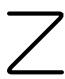
\includegraphics[keepaspectratio]{images/part001_3ab49149.jpg}}

\begin{enumerate}
\def\labelenumi{\arabic{enumi})}
\setcounter{enumi}{1}
\tightlist
\item
  设 \(\mathfrak{g} \subset \mathfrak{gl}(V)\)，\(\mathfrak{g}' \subset \mathfrak{gl}(V')\) 是可分解李代数，\(\varphi\) 是 \(\mathfrak{g}\) 到 \(\mathfrak{g}'\) 的一个同构。注意，\(\varphi\) 未必把 \(\mathfrak{g}\) 的半单（相应地，幂零）元素变为 \(\mathfrak{g}'\) 的半单（相应地，幂零）元素（习题 2）。然而，若 \(\mathfrak{g}\) 半单，则情形就是如此（第一章，§6，第 3 节，定理 3）。
\end{enumerate}

命题 3. 设 \(\mathfrak{a}\) 是 \(\mathfrak{gl}(\mathrm{V})\) 的一个可分解李子代数，并设 \(\mathfrak{b}\) 与 \(\mathfrak{c}\) 是 \(\mathfrak{gl}(\mathrm{V})\) 的向量子空间，满足 \(\mathfrak{b} \subset \mathfrak{c}\)。设 \(\mathfrak{a}'\) 是那些 \(x \in \mathfrak{a}\)（满足 \([x, \mathfrak{c}] \subset \mathfrak{b}\)）所成的集。则 \(\mathfrak{a}'\) 是可分解的。

置 \(\mathfrak{g} = \mathfrak{gl}(\mathrm{V})\)；子代数 \(\mathfrak{h}'\)（\(\mathfrak{gl}(\mathfrak{g})\) 中由那些 \(z \in \mathfrak{gl}(\mathfrak{g})\)（满足 \(z(\mathfrak{c}) \subset \mathfrak{b}\)）组成的）是可分解的（例 1）。设 \(\pi : \mathfrak{g} \to \mathfrak{gl}(\mathfrak{g})\) 是 \(\mathfrak{g}\) 的伴随表示。把命题 2 (iv) 应用于 \(\pi\)，表明 \(\pi^{-1}(\mathfrak{h}')\) 是可分解的。因而 \(\mathfrak{a}' = \mathfrak{a} \cap \pi^{-1}(\mathfrak{h}')\) 也是可分解的。

推论 1. 若 \(\mathfrak{a}\) 是 \(\mathfrak{gl}(\mathrm{V})\) 的一个可分解李子代数，且 \(\mathfrak{n}\) 是 \(\mathfrak{a}\) 的一个李子代数，则 \(\mathfrak{n}\) 在 \(\mathfrak{a}\) 中的正规化子（相应地，中心化子）是可分解的。

这由命题 3 取 \(\mathfrak{c} = \mathfrak{n},\mathfrak{b} = \mathfrak{n}\)（相应地，\(\mathfrak{c} = \mathfrak{n},\mathfrak{b} = \{0\}\)）得到。

推论 2. \(\mathfrak{gl}(\mathrm{V})\) 的一个可分解李子代数的嘉当子代数都是可分解的。

这由推论 1 得出。

注记. 我们将在后面（第 5 节，定理 2）证明推论 2 的一个逆命题。

\subsection{可分解包络}

\(\mathfrak{gl}(V)\) 的一族可分解李子代数的交显然是可分解的。因而，若 g 是 \(\mathfrak{gl}(V)\) 的一个李子代数，则 \(\mathfrak{gl}(V)\) 的包含 g 的可分解李子代数所成的集有一个最小元素，称为 g 的可分解包络；在本节中，这个包络将记作 \(e(\mathfrak{g})\)。

命题 4. 设 \(\mathfrak{g}\) 是 \(\mathfrak{gl}(\mathrm{V})\) 的一个李子代数，\(\mathfrak{n}\) 是 \(\mathfrak{g}\) 的一个理想。则 \(\mathfrak{n}\) 与 \(e(\mathfrak{n})\) 都是 \(e(\mathfrak{g})\) 的理想，且 \([e(\mathfrak{g}), e(\mathfrak{n})] = [\mathfrak{g}, \mathfrak{n}]\)。

设 \(\mathfrak{g}_1\) 是那些 \(x\in \mathfrak{gl}(\mathrm{V})\)（满足 \([x,\mathfrak{n}]\subset [\mathfrak{g},\mathfrak{n}]\)）所成的集。这是 \(\mathfrak{gl}(\mathrm{V})\) 的一个可分解李子代数，包含 \(\mathfrak{g}\)，从而包含 \(e(\mathfrak{g})\)，参见第 1 节命题 3；换言之，\([e(\mathfrak{g}),\mathfrak{n}]\subset [\mathfrak{g},\mathfrak{n}]\)。设 \(\mathfrak{n}_1\) 是那些 \(y\in \mathfrak{gl}(\mathrm{V})\) 所成的集，使得

\[
[ e (\mathfrak {g}), y ] \subset [ \mathfrak {g}, \mathfrak {n} ].
\]

由前所述，这是 \(\mathfrak{gl}(V)\) 的一个包含 n 的可分解李子代数，从而包含 \(e(\mathfrak{n})\)；换言之，\([e(\mathfrak{g}), e(\mathfrak{n})] \subset [\mathfrak{g}, \mathfrak{n}]\)，于是

\[
[ e (\mathfrak {g}), e (\mathfrak {n}) ] = [ \mathfrak {g}, \mathfrak {n} ].
\]

由此推出 \([e(\mathfrak{g}),\mathfrak{n}]\subset [e(\mathfrak{g}),e(\mathfrak{n})]\subset \mathfrak{n}\)，于是 \(\mathfrak{n}\) 与 \(e(\mathfrak{n})\) 都是 \(e(\mathfrak{g})\) 的理想。

推论 1. (i) \(\mathcal{D}^i\mathfrak{g} = \mathcal{D}^i e(\mathfrak{g})\) 对 \(i\geq 1\) 成立，且 \(\mathcal{C}^i\mathfrak{g} = \mathcal{C}^i e(\mathfrak{g})\) 对 \(i\geq 2\) 成立。

\begin{enumerate}
\def\labelenumi{(\roman{enumi})}
\setcounter{enumi}{1}
\tightlist
\item
  若 g 交换（相应地，幂零、可解），则 \(e(\mathfrak{g})\) 交换（相应地，幂零、可解）。
\end{enumerate}

断言 (i) 由命题 4 对 i 用归纳法得到，而 (ii) 由 (i) 得到。

推论 2. 设 \(\mathfrak{r}\) 是 \(\mathfrak{g}\) 的根基。若 \(\mathfrak{g}\) 可分解，则 \(\mathfrak{r}\) 可分解。

事实上，由命题 4 与推论 1，\(e(\mathfrak{r})\) 是 \(\mathfrak{g}\) 的一个可解理想，故 \(e(\mathfrak{r}) = \mathfrak{r}\)。

\subsection{可分解代数的分解}

若 g 是 \(\mathfrak{gl}(V)\) 的一个李代数（具有根基 r），则 r 的幂零元素所成的集是 g 的一个幂零理想，即 g 的恒等表示的最大幂零性理想（第一章，§5，第 3 节，定理 1 的推论 6）。在本节中，我们将把这个理想记作 \(\mathfrak{n}_{\mathrm{V}}(\mathfrak{g})\)。它包含 g 的幂零根基 \([g,g]\cap r\)（第一章，§5，第 3 节，定理 1）。

命题 5. 设 g 是 \(\mathfrak{gl}(V)\) 的一个可分解幂零李子代数。设 t 是 g 的半单元素所成的集。则 t 是 g 的一个中心子代数，且 g 作为李代数是 t 与 \(\mathfrak{n}_{\mathrm{V}}(\mathfrak{g})\) 的积。

若 \(x \in t\)，则 \(ad_{g}x\) 既半单又幂零，故为零，从而 x 在 g 中是中心的。因而 t 是 g 的一个理想，且 \(t \cap \mathfrak{n}_{\mathrm{V}}(\mathfrak{g}) = 0\)。由于 g 可分解，\(\mathfrak{g} = \mathfrak{t} + \mathfrak{n}_{\mathrm{V}}(\mathfrak{g})\)，命题得证。

命题 6. 设 g 是 \(\mathfrak{gl}(\mathrm{V})\) 的一个可分解李子代数。设 T 是由半单元素组成的 g 的交换子代数所成的集，\(T_{1}\) 是 T 的极大元素所成的集。设 H 是 g 的嘉当子代数所成的集。

\begin{enumerate}
\def\labelenumi{(\roman{enumi})}
\item
  对 \(\mathfrak{h} \in \mathcal{H}\)，设 \(\varphi(\mathfrak{h})\) 是 \(\mathfrak{h}\) 的半单元素所成的集。则 \(\varphi(\mathfrak{h}) \in \mathcal{T}_1\)。
\item
  对 \(\mathfrak{t} \in \mathcal{T}_1\)，设 \(\psi(\mathfrak{t})\) 是 \(\mathfrak{t}\) 在 \(\mathfrak{g}\) 中的交换子。则 \(\psi(\mathfrak{t}) \in \mathscr{H}\)。
\item
  映射 \(\varphi\) 与 \(\psi\) 分别是从 \(\mathcal{H}\) 到 \(\mathcal{T}_1\) 与从 \(\mathcal{T}_1\) 到 \(\mathcal{H}\) 的互逆双射。
\item
  若 \(k\) 代数闭，则 \(\mathrm{Aut}_e(\mathfrak{g})\) 传递地作用于 \(\mathcal{T}_1\)。
\end{enumerate}

设 \(\mathfrak{h} \in \mathcal{H}\)，并置 \(\mathfrak{t} = \varphi(\mathfrak{h})\)。由命题 5 与命题 3 的推论 2，\(\mathfrak{t} \in \mathcal{T}\) 且 \(\mathfrak{h} = \mathfrak{t} \times \mathfrak{n}_{\mathrm{V}}(\mathfrak{h})\)。对任何子代数 \(\mathfrak{u}\)（\(\mathfrak{g}\) 的子代数），用 \(\psi(\mathfrak{u})\) 表示 \(\mathfrak{u}\) 在 \(\mathfrak{g}\) 中的交换子。则 \(\mathfrak{h} \subset \psi(\mathfrak{t})\)，且 \(\psi(\mathfrak{t}) \subset \mathfrak{g}^0(\mathfrak{h})\)，因为 \(\mathfrak{n}_{\mathrm{V}}(\mathfrak{h})\) 的元素都是幂零的，故 \(\mathfrak{h} = \psi(\mathfrak{t})\)。若 \(\mathfrak{t}' \in \mathcal{T}\) 且 \(\mathfrak{t} \subset \mathfrak{t}'\)，则 \(\mathfrak{t}' \subset \psi(\mathfrak{t}) = \mathfrak{h}\)，于是 \(\mathfrak{t}' = \mathfrak{t}\)，因而 \(\mathfrak{t} \in \mathcal{T}_1\)。

设 \(\mathfrak{t} \in \mathcal{T}_1\)，并置 \(\mathfrak{c} = \psi(\mathfrak{t})\)。设 \(\mathfrak{h}\) 是 \(\mathfrak{c}\) 的一个嘉当子代数。由 §2 第 3 节命题 10，\(\mathfrak{h} \in \mathcal{H}\) 且 \(\mathfrak{t} \subset \mathfrak{h}\)。置 \(\mathfrak{t}_1 = \varphi(\mathfrak{h}) \in \mathcal{T}\)。则 \(\mathfrak{t} \subset \mathfrak{t}_1\)，故 \(\mathfrak{t} = \mathfrak{t}_1\)，且由前所述 \(\mathfrak{h} = \psi(\mathfrak{t}_1) = \psi(\mathfrak{t}) = \mathfrak{c}\)。于是 \(\psi(\mathfrak{t}) \in \mathcal{H}\)，且 \(\varphi(\psi(\mathfrak{t})) = \mathfrak{t}\)。

我们就这样证明了 (i)、(ii) 与 (iii)。设 \(k\) 代数闭。由于 \(\mathrm{Aut}_e(\mathfrak{g})\) 传递地作用于 \(\mathcal{H}(\S 3, \text{no. } 2, \text{Th. } 1)\)，故 \(\mathrm{Aut}_e(\mathfrak{g})\) 传递地作用于 \(\mathcal{T}_1\)。

推论 1. \(\mathfrak{g}\) 的嘉当子代数是 \(\mathfrak{g}\) 的正则半单元素的中心化子。

若 \(x \in \mathfrak{g}\) 正则，则 \(\mathfrak{g}^0(x)\) 是 \(\mathfrak{g}\) 的一个嘉当子代数（§2，第 3 节，定理 1 (i)）；此外，若 \(x\) 半单，则 \(\mathfrak{g}^0(x)\) 是 \(x\) 在 \(\mathfrak{g}\) 中的中心化子。反之，设 \(\mathfrak{h}\) 是 \(\mathfrak{g}\) 的一个嘉当子代数。存在 \(\mathfrak{t} \in \mathcal{T}_1\)，使得 \(\mathfrak{h} = \psi(\mathfrak{t})\)。由 §1 第 2 节命题 7，存在 \(x \in \mathfrak{t}\)，使得 \(\mathfrak{h} = \mathfrak{g}^0(x)\)；由于 \(x \in \mathfrak{t}\)，\(\mathfrak{g}^0(x) = \mathfrak{g}_0(x)\)。由 §3 第 3 节定理 2 (ii)，\(x\) 正则。

推论 2. 再设 g 可解。则：

\begin{enumerate}
\def\labelenumi{(\roman{enumi})}
\item
  \(\operatorname{Aut}(\mathfrak{g})\) 中由诸 \(e^{\mathrm{ad}x}, x \in \mathcal{C}^{\infty}\mathfrak{g}\)（参见 §3 第 4 节）组成的子群传递地作用于 \(\mathcal{T}_1\)。
\item
  若 \(\mathfrak{t} \in \mathcal{T}_1\)，则 \(\mathfrak{g}\) 是 \(\mathfrak{t}\) 与 \(\mathfrak{n}_{\mathrm{V}}(\mathfrak{g})\) 的半直积。
\end{enumerate}

断言 (i) 由下列事实得出：诸 \(e^{\mathrm{ad}x}\)（\(x \in \mathcal{C}^{\infty}\mathfrak{g}\)）所成的群传递地作用于 \(\mathcal{H}(\S 3\)，第 4 节，定理 3）。

我们证明 (ii)。设 \(t \in T_{1}\)，并设 \(\mathfrak{h} = \psi(t)\) 是 g 的相应的嘉当子代数。鉴于命题 5，\(\mathfrak{h} = \mathfrak{t} + \mathfrak{n}_{\mathrm{V}}(\mathfrak{h}) \subset \mathfrak{t} + \mathfrak{n}_{\mathrm{V}}(\mathfrak{g})\)。另一方面，\(g = h + [g, g]\)（§2，第 1 节，命题 4 的推论 3）且 \([\mathfrak{g}, \mathfrak{g}] \subset \mathfrak{n}_{\mathrm{V}}(\mathfrak{g})\)，故 \(\mathfrak{g} = \mathfrak{t} + \mathfrak{n}_{\mathrm{V}}(\mathfrak{g})\)。但显然 \(\mathfrak{t} \cap \mathfrak{n}_{\mathrm{V}}(\mathfrak{g}) = \{0\}\)。于是代数 g 是 t 与理想 \(\mathfrak{n}_{\mathrm{V}}(\mathfrak{g})\) 的半直积。

命题 7. 设 \(\mathfrak{g}\) 是 \(\mathfrak{gl}(\mathrm{V})\) 的一个可分解李子代数。

\begin{enumerate}
\def\labelenumi{(\roman{enumi})}
\item
  存在一个李子代数 \(\mathfrak{m}\)（\(\mathfrak{g}\) 的李子代数），它在 \(\mathfrak{gl}(\mathrm{V})\) 中约化，使得 \(\mathfrak{g}\) 是 \(\mathfrak{m}\) 与 \(\mathfrak{n}_{\mathrm{V}}(\mathfrak{g})\) 的半直积。
\item
  \(\mathfrak{g}\) 的任何两个具有 (i) 中性质的李子代数都在 \(\mathrm{Aut}_e(\mathfrak{g})\) 下共轭。
\end{enumerate}

g 的根基 r 可分解（第 2 节，命题 4 的推论 2）。由命题 6 的推论 2，存在 r 的一个由半单元素组成的交换子代数 t，使得 \(\mathfrak{r} = \mathfrak{t} \oplus \mathfrak{n}_{\mathrm{V}}(\mathfrak{r})\)。由于 \(ad_{g}t\) 由半单元素组成，g 是 \([t, g]\) 与 t 的中心化子 z 的直和（第一章，§3，第 5 节，命题 6）。由于 \([t, g] \subset r\)，\(g = z + r\)。因而，若 s 是 z 的一个 Levi 子代数（第一章，§6，第 8 节），则 \(g = s + r\)，故 s 是 g 的一个 Levi 子代数。置 \(m = s \oplus t\)。由于 \([s, t] = \{0\}\)，m 是 g 的一个李子代数，且由第一章 §6 第 5 节定理 4，它在 \(\mathfrak{gl}(V)\) 中约化。此外，

\[
\mathfrak {g} = \mathfrak {s} \oplus \mathfrak {r} = \mathfrak {s} \oplus \mathfrak {t} \oplus \mathfrak {n} _ {\mathrm{V}} (\mathfrak {r}) = \mathfrak {s} \oplus \mathfrak {t} \oplus \mathfrak {n} _ {\mathrm{V}} (\mathfrak {g}) = \mathfrak {m} \oplus \mathfrak {n} _ {\mathrm{V}} (\mathfrak {g})
\]

因为 \(\mathfrak{n}_{\mathrm{V}}(\mathfrak{g}) = \mathfrak{n}_{\mathrm{V}}(\mathfrak{r})\)。故得 (i)。

现在设 \(\mathfrak{m}'\) 是 \(\mathfrak{g}\) 的一个李子代数，它是 \(\mathfrak{n}_{\mathrm{V}}(\mathfrak{g})\) 的补，且在 \(\mathfrak{gl}(\mathrm{V})\) 中约化。我们证明 \(\mathfrak{m}'\) 与 \(\mathfrak{m}\) 在 \(\operatorname{Aut}_e(\mathfrak{g})\) 下共轭。我们有 \(\mathfrak{m}' = \mathfrak{s}' \oplus \mathfrak{t}'\)，其中 \(\mathfrak{s}' = [\mathfrak{m}', \mathfrak{m}']\) 半单，且中心 \(\mathfrak{t}'\)（\(\mathfrak{m}'\) 的中心）由半单元素组成。则 \(\mathfrak{r} = \mathfrak{t} \oplus \mathfrak{n}_{\mathrm{V}}(\mathfrak{g}) = \mathfrak{t}' \oplus \mathfrak{n}_{\mathrm{V}}(\mathfrak{g})\)。鉴于命题 6 的推论 2，我们化为情形 \(\mathfrak{t} = \mathfrak{t}'\)。则 \(\mathfrak{s}' \subset \mathfrak{z}\)；由于 \(\dim \mathfrak{s}' = \dim \mathfrak{s}\)，\(\mathfrak{s}'\) 是 \(\mathfrak{z}\) 的一个 Levi 子代数。由第一章 §6 第 8 节定理 5，存在 \(x \in \mathfrak{n}_{\mathrm{V}}(\mathfrak{z})\)，使得 \(e^{\operatorname{ad} x}(\mathfrak{s}) = \mathfrak{s}'\)；由于 \(x\) 与 \(\mathfrak{t}\) 交换，还有 \(e^{\operatorname{ad} x}(\mathfrak{t}) = \mathfrak{t}\)。

\subsection{幂零自同态的线性李代数}

引理 1. 设 \(\mathfrak{n}\) 是 \(\mathfrak{gl}(\mathrm{V})\) 的一个由幂零自同态组成的李子代数，\(\mathrm{N}\) 是子群 \(\exp \mathfrak{n}\)（\(\mathbf{GL}(\mathrm{V})\) 的子群）（§3，第 1 节，引理 1）。

\begin{enumerate}
\def\labelenumi{(\roman{enumi})}
\item
  设 \(\rho\) 是 \(\mathfrak{n}\) 在 W 上的一个有限维线性表示，使得 \(\rho(\mathfrak{n})\) 的元素都是幂零的，W' 是 W 的一个在 \(\rho\) 下稳定的向量子空间，\(\rho_1\) 与 \(\rho_2\) 是由 W' 定义的 \(\rho\) 的子表示与商表示，\(\pi, \pi_1, \pi_2\) 是与 \(\rho, \rho_1, \rho_2\) 相容的 N 的表示（§3，第 1 节）。则 \(\pi_1, \pi_2\) 是由 W' 定义的 \(\pi\) 的子表示与商表示。
\item
  设 \(\rho_1, \rho_2\) 是 \(\mathfrak{n}\) 的有限维线性表示，使得 \(\rho_1(\mathfrak{n})\) 与 \(\rho_2(\mathfrak{n})\) 的元素都是幂零的，\(\pi_1, \pi_2\) 是与 \(\rho_1, \rho_2\) 相容的 N 的表示。则 \(\pi_1 \otimes \pi_2\) 是与 \(\rho_1 \otimes \rho_2\) 相容的 N 的表示。
\item
  设 \(\rho_{1},\rho_{2}\) 是 \(\mathfrak{n}\) 在向量空间 \(V_{1},V_{2}\) 上的有限维线性表示，使得 \(\rho_1(\mathfrak{n})\) 与 \(\rho_{2}(\mathfrak{n})\) 的元素都是幂零的，\(\rho\) 是 \(\mathfrak{n}\) 在 \(\mathrm{Hom}(V_1,V_2)\) 上由 \(\rho_{1},\rho_{2}\) 确定的表示。设 \(\pi_1,\pi_2\) 是与 \(\rho_{1},\rho_{2}\) 相容的 N 的表示，\(\pi\) 是 N 在 \(\mathrm{Hom}(\mathrm{V}_1,\mathrm{V}_2)\) 上由 \(\pi_1,\pi_2\) 确定的表示。则 \(\pi\) 是与 \(\rho\) 相容的 N 的表示。
\end{enumerate}

断言 (i) 是明显的。设 \(\rho_1, \rho_2, \pi_1, \pi_2\) 如 (ii) 中所述。若 \(x \in \mathfrak{n}\)，则由于 \(\rho_1(x) \otimes 1\) 与 \(1 \otimes \rho_2(x)\) 交换，我们有

\[
\begin{array}{l} \exp (\rho_ {1} (x) \otimes 1 + 1 \otimes \rho_ {2} (x)) = \exp (\rho_ {1} (x) \otimes 1). \exp (1 \otimes \rho_ {2} (x)) \\ \qquad = (\exp \rho_ {1} (x)) \otimes 1. 1 \otimes (\exp \rho_ {2} (x)) \\ \qquad = (\exp \rho_ {1} (x)) \otimes (\exp \rho_ {2} (x)) \\ \qquad = \pi_ {1} (\exp x) \otimes \pi_ {2} (\exp x) \\ \qquad = (\pi_ {1} \otimes \pi_ {2}) (\exp x), \end{array}
\]

故得 (ii)。设 \(\rho_1, \rho_2, \rho, \pi_1, \pi_2, \pi, V_1, V_2\) 如 (iii) 中所述。若 \(v_1 \in \mathrm{End}V_1\) 且 \(v_2 \in \mathrm{End}V_2\)，用 \(R_{v_1}\) 与 \(L_{v_2}\) 表示映射 \(u \mapsto uv_1\) 与 \(u \mapsto v_2u\)（从 \(\mathrm{Hom}(V_1, V_2)\) 到自身的映射）；这些映射交换，且 \(\rho(x)u = (L_{\rho_2(x)} - R_{\rho_1(x)})u\)，于是

\[
\begin{array}{r l} & {\exp \rho (x). u = \exp \mathrm{L} _ {\rho_ {2} (x)}. \exp \mathrm{R} _ {- \rho_ {1} (x)}. u} \\ & {\qquad = \mathrm{L} _ {\exp \rho_ {2} (x)}. \mathrm{R} _ {\exp (- \rho_ {1} (x))}. u} \\ & {\qquad = \mathrm{L} _ {\pi_ {2} (\exp x)}. \mathrm{R} _ {\pi_ {1} (\exp (- x))}. u} \\ & {\qquad = \pi (\exp x). u,} \end{array}
\]

故得 (iii)。

引理 2 \(^{2}\). (i) 设 W 是 V 的一个维数为 d 的向量子空间，D 是直线 \(\bigwedge^{d}\) W \(\subset \bigwedge^{d}\) V，\(\theta\) 是 \(\mathfrak{gl}(V)\) 在 \(\bigwedge V\) 上的典则表示（第三章，附录）。设 \(x \in \mathfrak{gl}(V)\)。则 \(x(W) \subset W\) 当且仅当 \(\theta(x)(D) \subset D\)。

\begin{enumerate}
\def\labelenumi{(\roman{enumi})}
\setcounter{enumi}{1}
\tightlist
\item
  设 \((e_{1},\ldots,e_{n})\) 是 \(k^{n}\) 的典则基，\(\theta\) 是 \(\mathfrak{gl}(n,k)\) 在 \(\bigwedge(k^{n})\) 上的典则表示，\(x\in\mathfrak{gl}(n,k)\)。则 \(x\in\mathfrak{n}(n,k)\) 当且仅当
\end{enumerate}

\[
\theta (x) (e _ {n - d + 1} \wedge \dots \wedge e _ {n}) = 0
\]

对所有 \(1 \leq d \leq n\) 成立。

\footnotetext[2]{在这个引理中，\(k\) 可以是任意（交换）域。}

\begin{enumerate}
\def\labelenumi{(\roman{enumi})}
\tightlist
\item
  若 \(x(\mathrm{W}) \subset \mathrm{W}\)，则显然 \(\theta(x)\mathrm{D} \subset \mathrm{D}\)。反之，设 \(\theta(x)\mathrm{D} \subset \mathrm{D}\)。设 \(u\) 是 \(\mathrm{D}\) 的一个非零元素，并设 \(y \in \mathrm{W}\)。则 \(y \wedge u = 0\)。由于 \(\theta(x)\) 是 \(\bigwedge \mathrm{V}\) 的一个导子，这蕴含
\end{enumerate}

\[
\theta (x) y \wedge u + y \wedge \theta (x) u = 0.
\]

而现在 \(\theta(x)u\in ku\)，故 \(y\wedge\theta(x)u=0\)，从而 \(\theta(x)y\wedge u=0\)。由《代数》第三章 §7 第 9 节命题 13，这蕴含 \(\theta(x)y\in W\)，即 \(x(y)\in W\)，这就证明 \(x(W)\subset W\)。

\begin{enumerate}
\def\labelenumi{(\roman{enumi})}
\setcounter{enumi}{1}
\tightlist
\item
  对 \(x \in \mathfrak{n}(n, k)\) 而言，(ii) 中所述的条件显然是必要的。设它成立。由 (i)，\(x\) 使
\end{enumerate}

\[
k e _ {n - d + 1} + \dots + k e _ {n}
\]

保持稳定，又由于这对 \(d = 1, \ldots, n\) 都成立，\(x\) 是下三角的。置

\[
x = (x _ {i j}) _ {1 \leq i, j \leq n}.
\]

我们有 \(0 = x(e_n) = x_{nn}e_n\)，故 \(x_{nn} = 0\)。设 \(i < n\)，并设已证明 \(x_{jj} = 0\) 对 \(j > i\) 成立。则

\[
0 = \theta (x) \left(e _ {i} \wedge e _ {i + 1} \wedge \dots \wedge e _ {n}\right) = x _ {i i} \left(e _ {i} \wedge e _ {i + 1} \wedge \dots \wedge e _ {n}\right),
\]

故 \(x_{ii} = 0\)。于是 \(x \in \mathfrak{n}(n,k)\)。

命题 8. 设 \(\mathfrak{n}\) 是 \(\mathfrak{gl}(\mathrm{V})\) 的一个由幂零元素组成的李子代数，\(\mathfrak{q}\) 是 \(\mathfrak{n}\) 在 \(\mathfrak{gl}(\mathrm{V})\) 中的正规化子。存在一个有限维向量空间 E、一个表示 \(\rho\)（\(\mathfrak{gl}(\mathrm{V})\) 在 E 上的表示）以及 E 的一个向量子空间 F，满足下列条件：

\begin{enumerate}
\def\labelenumi{(\roman{enumi})}
\item
  在 \(\rho\) 下，\(V\) 的位似的像是可对角化的；
\item
  F 在 \(\rho(\mathfrak{q})\) 下稳定；
\item
  \(\mathfrak{n}\) 是那些 \(x\in \mathfrak{gl}(\mathrm{V})\)（满足 \(\rho (x)(\mathrm{F}) = 0\)）所成的集
\end{enumerate}

设 \(n = \dim V\)。由 Engel 定理，可以把 \(V\) 与 \(k^n\) 等同起来，使得 \(\mathfrak{n} \subset \mathfrak{n}(n,k)\)。设 \(P\) 是 \(\mathfrak{gl}(n,k)\) 上的多项式函数所成的代数。对 \(i = 0,1,\ldots\)，设 \(P_i\) 是 \(P\) 中 \(i\) 次齐次元素所成的集。设 \(N = \exp \mathfrak{n}\)，它是严格下三角群 \(T\) 的一个子群。设 \(J\) 是 \(P\) 中在 \(N\) 上为零的元素所成的集；这是 \(P\) 中的一个理想。设 \(N_J\) 是那些 \(x \in \mathfrak{gl}(n,k)\)（使得 \(p(x) = 0\) 对所有 \(p \in J\) 成立）所成的集。则 \(N \subset N_J\)。反之，设 \(x \in N_J\)。用 \(p_{ij}\) 表示给出 \(\mathfrak{gl}(n,k)\) 的一个元素的矩阵项的多项式函数。理想 \(J\) 含有诸 \(p_{ij}\)（对 \(i < j\)）与诸 \(p_{ii} - 1\)；因而 \(x \in T\)。另一方面，若 \(u\) 是 \(\mathfrak{gl}(n,k)\) 上的一个在 \(\mathfrak{n}\) 上为零的线性形式，则存在 \(p_u \in P\)，使得 \(p_u(z) = u(\log z)\) 对所有 \(z \in T\) 成立（\(\S 3\)，第 1 节，引理 1 (i)）；我们有 \(p_u \in J\)，故 \(u(\log x) = 0\)。由此推出 \(\log x\) 属于 \(\mathfrak{n}\)，于是 \(x \in N\)，这就证明了 \(N = N_J\)。

对所有 \(p \in P\) 与 \(g \in \mathbf{GL}_{n}(k)\)，设 \(\lambda(g)p\) 是函数 \(x \mapsto p(g^{-1}x)\)（\(\mathfrak{gl}(n,k)\) 上的函数）；则 \(\lambda(g)p \in \mathrm{P}\)，\(\lambda(g)\) 是代数 P 的一个自同构，且 \(\lambda\) 是 \(\mathbf{GL}_{n}(k)\) 在 P 上的一个表示，它使每个 \(P_{i}\) 保持稳定。我们证明

\[
\mathrm{N} = \{x \in \mathbf {G L} _ {n} (k) \mid \lambda (x) \mathrm{J} = \mathrm{J} \}.\tag{1}
\]

若 \(x \in \mathrm{N}, p \in \mathrm{J}, y \in \mathrm{N}\)，则 \((\lambda(x)p)(y) = p(x^{-1}y) = 0\)，因为 \(x^{-1}y \in \mathrm{N}\)；于是 \(\lambda(x)p \in \mathrm{J}\)，故 \(\lambda(x)\mathrm{J} = \mathrm{J}\)。设 \(x \in \mathbf{GL}_n(k)\) 满足 \(\lambda(x)\mathrm{J} = \mathrm{J}\)；设 \(p \in \mathrm{J}\)；则 \(p(x^{-1}) = (\lambda(x)p)(e) = 0\)，故 \(x^{-1} \in \mathrm{N}_{\mathrm{J}} = \mathrm{N}\) 且 \(x \in \mathrm{N}\)。这就证明了 (i)。

理想 J 是有限型的（《交换代数》，第三章，§2，第 10 节，定理 2 的推论 2）。因而，存在一个整数 q，使得若 \(W = P_{0} + P_{1} + \cdots + P_{q}\)，则 \(J \cap W\) 作为理想生成 J。用 \(\lambda_{j}\)（相应地，\(\lambda'\)）表示 \(\lambda\) 的由 \(P_{J}\)（相应地，由 W）定义的子表示。由 (1)，

\[
\mathrm{N} = \{x \in \mathbf {G L} _ {n} (k) \mid \lambda^ {\prime} (x) (\mathrm{J} \cap \mathrm{W}) = \mathrm{J} \cap \mathrm{W} \}.\tag{2}
\]

我们证明，对所有 \(j\)，存在表示 \(\sigma_{j}\)（李代数 \(\mathfrak{gl}(n,k)\) 在 \(\mathrm{P}_j\) 上的表示），使得：

\[
\sigma_ {j} | \mathfrak {n} (n, k) \text {   is   compatible   } (\S 3, \text {   no.   } 1) \text {   with   } \lambda_ {j} | T.\tag{3}
\]

\[
\text { For   all } x \in k. 1 _ {n}, \sigma_ {j} (x) \text { is   a   homothety. }\tag{4}
\]

由于 \(\lambda_{j}\) 是 \(\lambda_{1}\) 的第 j 个对称幂，只需证明 \(\sigma_{1}\) 的存在性，参见引理 1。现在 \(\lambda_{1}\) 是表示 \(\gamma\)（\(\mathbf{GL}_{n}(k)\) 在 \(\mathfrak{gl}(n,k)\) 上的表示）的反步表示，由下式给出

\[
\gamma (x) y = x y, \quad x \in \mathbf {G L} _ {n} (k), \quad y \in \mathfrak {g l} (n, k).
\]

设 \(c\) 是李代数 \(\mathfrak{gl}(n,k)\) 在 \(\mathfrak{gl}(n,k)\) 上的表示，由下式给出

\[
c (x) y = x y, \quad x, y \in \mathfrak {g l} (n, k).
\]

直接看出 \(c|\mathfrak{n}(n,k)\) 与 \(\gamma|T\) 相容，且 \(c(x)\) 对所有 \(x \in k.1_{n}\) 是位似。于是，只需取 \(\sigma_{1}\) 为 c 的对偶表示（第一章，§3，第 3 节）。

现在设 \(\sigma'\) 是 \(\mathfrak{gl}(n,k)\) 在 W 上的表示，由诸 \(\sigma_j\)（\(0 \leq j \leq q\)）的直和给出。鉴于 (2) 与关系式

\[
\lambda^ {\prime} (\exp (x)) = \exp (\sigma^ {\prime} (x)) \text { and } \sigma^ {\prime} (\log (y)) = \log (\lambda^ {\prime} (y)), x \in \mathfrak {n} (n, k), y \in \mathrm{T},
\]

我们有

\[
\mathfrak {n} = \{x \in \mathfrak {n} (n, k) \mid \sigma^ {\prime} (x) (\mathrm{J} \cap \mathrm{W}) \subset \mathrm{J} \cap \mathrm{W} \}.\tag{5}
\]

设 \(d = \dim(\mathrm{J} \cap \mathrm{W})\)，并设 \(\tau = \bigwedge^{d} \sigma'\)。设 \(\mathrm{D} = \bigwedge^{d} (\mathrm{J} \cap \mathrm{W})\)。由 (5) 与引理 2 (i)，

\[
\mathfrak {n} = \{x \in \mathfrak {n} (n, k) \mid \tau (x) (\mathrm{D}) \subset \mathrm{D} \}.\tag{6}
\]

但 \(\tau (\mathfrak{n}(n,k))\) 由幂零自同态组成，故 (6) 也可写成

\[
\mathfrak {n} = \{x \in \mathfrak {n} (n, k) \mid \tau (x) (\mathrm{D}) = 0 \}.\tag{7}
\]

现在设 \(E = \bigwedge^{d} W \oplus \bigwedge^{1} V \oplus \bigwedge^{2} V \oplus \cdots \oplus \bigwedge^{n} V\)；设 \(\rho\) 是 \(\tau\) 与 \(\mathfrak{gl}(n, k)\) 在 \(\bigwedge^{1} V, \ldots, \bigwedge^{n} V\) 上的典则表示的直和。设 \(E_{0} \subset E\) 是 \(D = \bigwedge^{d} (J \cap W)\) 与由 \(e_{n-j+1} \wedge \cdots \wedge e_{n}\)（对 \(j = 1, \ldots, n\)）生成的直线的和。由 (7) 与引理 2 (ii)，

\[
\mathfrak {n} = \{x \in \mathfrak {g l} (\mathrm{V}) \mid \rho (x) (\mathrm{E} _ {0}) = 0 \}.\tag{8}
\]

直接看出，若 \(x \in k.1_{n}\)，则 \(\rho(x)\) 可对角化。最后，若 F 是 E 中被 \(\rho(\mathfrak{n})\) 零化的元素所成的集，则 F 在 \(\rho(\mathfrak{q})\) 下稳定（第一章，§3，第 5 节，命题 5），且由 (8)，

\[
\mathfrak {n} = \{x \in \mathfrak {g l} (\mathrm{V}) \mid \rho (x) (\mathrm{F}) = 0 \}.\tag{9}
\]

\subsection{可分解李代数的特征刻画}

每个可分解李代数作为向量空间（更不必说作为李代数）由它的半单或幂零元素所成的集生成。反之：

定理 1. 设 g 是 \(\mathfrak{gl}(V)\) 的一个李子代数，并设 X 是 g 的一个子集，它把 g 生成为 k 上的李代数。若 X 的每个元素都是半单的或幂零的，则 g 可分解。

\begin{enumerate}
\def\labelenumi{\alph{enumi})}
\tightlist
\item
  \(\mathfrak{g}\) 交换。
\end{enumerate}

g 的半单（相应地，幂零）元素构成一个向量子空间 \(g_{s}\)（相应地，\(g_{n}\)）。假定等价于 \(g = g_{s} \oplus g_{n}\)，由此得到 g 可分解这一事实。

\begin{enumerate}
\def\labelenumi{\alph{enumi})}
\setcounter{enumi}{1}
\tightlist
\item
  \(\mathfrak{g}\) 是约化的。
\end{enumerate}

则 \(\mathfrak{g} = \mathfrak{g}' \times \mathfrak{c}\)，其中 \(\mathfrak{g}'\) 半单，\(\mathfrak{c}\) 交换。由命题 2，\(\mathfrak{g}'\) 可分解。设 \(x = a + b \in \mathfrak{g}\)，其中 \(a \in \mathfrak{g}'\)，\(b \in \mathfrak{c}\)。设 \(a_s, a_n, b_s, b_n\) 是 \(a, b\) 的半单分量与幂零分量。由于 \(a_s, a_n, b_s, b_n\) 相互交换，\(x\) 的半单分量与幂零分量是 \(a_s + b_s, a_n + b_n\)。而现在 \(a_s, a_n \in \mathfrak{g}'\)。若 \(x\) 半单，则 \(x = a_s + b_s\)；由于 \(a_s \in \mathfrak{g}'\)，有 \(b_s \in \mathfrak{g}\)，故 \(b_s \in \mathfrak{c}\)，因为 \(b_s\) 与 \(\mathfrak{g}\) 交换；因而 \(a = a_s\) 且 \(b = b_s\)。类似地，若 \(x\) 幂零，则 \(a = a_n\) 且 \(b = b_n\)。由此推出，X 的元素在 \(\mathfrak{c}\) 上的投影是半单的或幂零的；由 \(a)\)，这蕴含 \(\mathfrak{c}\) 可分解。保留前面的记号，但不加于 \(x\) 的假定，我们现在有 \(b_s, b_n \in \mathfrak{c}\)，于是 \(a_s + b_s, a_n + b_n \in \mathfrak{g}\)，这就证明了定理在这种情形下成立。

\begin{enumerate}
\def\labelenumi{\alph{enumi})}
\setcounter{enumi}{2}
\tightlist
\item
  一般情形。
\end{enumerate}

我们设定理对维数 \(< \dim \mathfrak{g}\) 的李代数已证明，并对 \(\mathfrak{g}\) 证明它。

设 \(\mathfrak{n}\) 是 \(\mathfrak{g}\) 的恒等表示的最大幂零性理想。若 \(\mathfrak{n} = 0\)，则 \(\mathfrak{g}\) 有一个单射半单表示，从而是约化的。设 \(\mathfrak{n} \neq 0\)。设 \(\mathfrak{p}\) 是 \(\mathfrak{n}\) 在 \(\mathfrak{gl}(\mathrm{V})\) 中的正规化子。存在满足命题 8 条件的 E、\(\rho, \mathrm{F}\)。由于 \(\mathfrak{g} \subset \mathfrak{p}\)，\(\rho(\mathfrak{g})\) 使 F 保持稳定；设 \(\rho_0\) 是表示 \(u \mapsto \rho(u)|\mathrm{F}\)（\(\mathfrak{g}\) 在 F 上的表示）；我们有 \(\mathfrak{n} = \mathrm{Ker}\rho_0\)。在 \(\rho\) 下，\(\mathfrak{gl}(\mathrm{V})\) 的每个半单（相应地，幂零）元素的像是半单的（相应地，幂零的）（命题 2）。于是代数 \(\rho_0(\mathfrak{g})\) 由它的半单元素与幂零元素生成。由归纳假设，\(\rho_0(\mathfrak{g})\) 可分解。

设 \(x \in \mathfrak{g}\)，并设 \(x_s, x_n\) 是它的半单分量与幂零分量。由命题 2，\(\rho(x)\) 的半单分量与幂零分量是 \(\rho(x_s), \rho(x_n)\)。由于 \(\rho_0(\mathfrak{g})\) 可分解，存在 \(y, z \in \mathfrak{g}\)，使得

\[
\rho_ {0} (y) = \rho (x _ {s}) | \mathrm{F}, \rho_ {0} (z) = \rho (x _ {n}) | \mathrm{F}.
\]

则 \(x_{s}\in y + \mathfrak{n},x_{n}\in z + \mathfrak{n}\)，故 \(x_{s},x_{n}\in \mathfrak{g}\)

证毕。

推论 1. \(\mathfrak{gl}(\mathrm{V})\) 的每个由它的可分解子代数生成的子代数都是可分解的。

这是明显的。

推论 2. 设 \(\mathfrak{g}\) 是 \(\mathfrak{gl}(\mathrm{V})\) 的一个李子代数。则 \([\mathfrak{g},\mathfrak{g}]\) 可分解。

设 \(\mathfrak{r}\) 是 \(\mathfrak{g}\) 的根基，\(\mathfrak{s}\) 是 \(\mathfrak{g}\) 的一个 Levi 子代数（第一章，§6，第 8 节）。则

\[
[ \mathfrak {g}, \mathfrak {g} ] = [ \mathfrak {s}, \mathfrak {s} ] + [ \mathfrak {s}, \mathfrak {r} ] + [ \mathfrak {r}, \mathfrak {r} ] = \mathfrak {s} + [ \mathfrak {g}, \mathfrak {r} ].
\]

代数 \([g,r]\) 可分解，因为它的所有元素都是幂零的（第一章，§5，第 3 节）。另一方面，s 可分解（命题 2）。由此推出 \([g,g]\) 可分解（推论 1）。

推论 3. 设 \(\mathfrak{g}\) 是 \(\mathfrak{gl}(\mathrm{V})\) 的一个李子代数，并设 \(\mathrm{X}\) 是 \(\mathfrak{g}\) 的一个生成 \(\mathfrak{g}\) 的子集（作为 \(k\) 上的李代数）。

\begin{enumerate}
\def\labelenumi{(\roman{enumi})}
\item
  可分解包络 \(e(\mathfrak{g})\)（\(\mathfrak{g}\) 的可分解包络）由 \(X\) 的元素的半单分量与幂零分量生成。
\item
  若 \(k'\) 是 \(k\) 的一个扩张，则 \(e(\mathfrak{g} \otimes_k k') = e(\mathfrak{g}) \otimes_k k'\)；且 \(\mathfrak{g}\) 可分解当且仅当 \(\mathfrak{g} \otimes_k k'\) 可分解。
\end{enumerate}

设 \(\tilde{\mathfrak{g}}\) 是 \(\mathfrak{gl}(\mathrm{V})\) 的由 X 的元素的半单分量与幂零分量生成的子代数。则 \(\mathfrak{g} \subset \tilde{\mathfrak{g}} \subset e(\mathfrak{g})\)；由定理 1，\(\tilde{\mathfrak{g}}\) 可分解，故 \(\tilde{\mathfrak{g}} = e(\mathfrak{g})\)，这就证明了 (i)。断言 (ii) 由此得出，因为 X 生成 \(k'\) -代数 \(\mathfrak{g} \otimes_k k'\)。

推论 4. 设 g 是 \(\mathfrak{gl}(\mathrm{V})\) 的一个可分解李子代数。设 T 是由半单元素组成的 g 的交换子代数所成的集（参见命题 6）。T 的极大元素都有相同的维数。

设 \(k'\) 是 \(k\) 的一个代数闭扩张，且 \(V' = V \otimes_k k', \mathfrak{g}' = \mathfrak{g} \otimes_k k'\)。设 \(t_1, t_2\) 是 \(\mathcal{T}\) 的极大元素，\(t_i' = t_i \otimes_k k'\)，\(\mathfrak{h}_i\) 是 \(t_i\) 在 \(\mathfrak{g}\) 中的交换子，\(\mathfrak{h}_i' = \mathfrak{h}_i \otimes_k k'\)。则 \(\mathfrak{h}_i\) 是 \(\mathfrak{g}\) 的一个嘉当子代数（命题 6），故 \(\mathfrak{h}_i'\) 是 \(\mathfrak{g}'\) 的一个嘉当子代数。于是 \(\mathfrak{h}_i = t_i \times \mathfrak{n}_V(\mathfrak{h}_i)\)，因而 \(\mathfrak{h}_i' = t_i' \times \mathfrak{n}_{V'}(\mathfrak{h}_i')\)，于是 \(t_i'\) 是 \(\mathfrak{h}_i'\) 的半单元素所成的集。由于 \(\mathfrak{g}'\) 可分解（推论 3），\(t_1'\) 与 \(t_2'\) 在 \(\text{Aut}_e(\mathfrak{g}')\) 下共轭（命题 6），故 \(\dim t_1 = \dim t_2\)。

定理 2. 设 \(\mathfrak{g}\) 是 \(\mathfrak{gl}(\mathrm{V})\) 的一个李子代数。下列条件等价：

\begin{enumerate}
\def\labelenumi{(\roman{enumi})}
\item
  \(\mathfrak{g}\) 可分解；
\item
  \(\mathfrak{g}\) 的每个嘉当子代数都可分解；
\item
  \(\mathfrak{g}\) 有一个可分解的嘉当子代数；
\item
  \(\mathfrak{g}\) 的根基可分解。
\item
  \(\Longrightarrow\) (ii)：这由命题 3 的推论 2 得出。
\item
  \(\Longrightarrow\) (i)：这由定理 1 的推论 1 得出，因为 \(\mathfrak{g}\) 由它的嘉当子代数生成（§2，第 3 节，定理 1 的推论 3）。
\item
  \(\Longrightarrow\) (iii)：这是明显的。
\item
  \(\Longrightarrow\) (ii)：由定理 1 的推论 3，可以设 k 代数闭。于是 g 的嘉当子代数在 g 的初等自同构下共轭（§3，第 2 节，定理 1）；鉴于 §3 第 1 节的注记 1，由此推出，若其中一个是可分解的，则它们全都是可分解的。
\item
  \(\Longrightarrow\) (iv)：这由命题 4 的推论 2 得出。
\item
  \(\Longrightarrow\) (i)：设 g 的根基 r 可分解。设 s 是 g 的一个 Levi 子代数；它可分解（命题 2）。因而 \(g = s + r\) 可分解（定理 1 的推论 1）。
\end{enumerate}

\appendixsection{多项式映射与 Zariski 拓扑}

在本附录中，设 \(k\) 是无限的。

\appendixitem{Zariski 拓扑}

设 V 是一个有限维向量空间。用 \(A_{V}\) 表示 V 上的以 k 为值的多项式函数所成的代数（《代数》，第四章，§5，第 10 节，定义 4）。这是一个分次代数；它的 1 次分量是 V 的对偶 \(V^{*}\)，且 \(V^{*}\) 到 \(A_{V}\) 中的单射扩张为对称代数 \(\mathbf{S}(V^{*})\) 到 \(A_{V}\) 的一个同构（《代数》，第四章，§5，第 11 节，注记 2）。

若 \((e_{1},\ldots,e_{n})\) 是 V 的一个基，且 \((\mathrm{X}_{1},\ldots,\mathrm{X}_{n})\) 是一个未定元序列，则从 \(k[\mathrm{X}_{1},\ldots,\mathrm{X}_{n}]\) 到 \(A_{V}\) 的映射把 \(k[\mathrm{X}_{1},\ldots,\mathrm{X}_{n}]\) 的任何元素 f 变为函数

\[
\sum_ {i = 1} ^ {n} \lambda_ {i} e _ {i} \mapsto f (\lambda_ {1}, \ldots , \lambda_ {n})
\]

是代数的一个同构（《代数》，第四章，§5，第 10 节，命题 19 的推论）。

命题 1. 设 H 是从 \(A_{V}\) 到 k 的代数同态所成的集。对任何 \(x \in V\)，设 \(h_{x}\) 是同态 \(f \mapsto f(x)\)（从 \(A_{V}\) 到 k 的同态）。则映射 \(x \mapsto h_{x}\) 是从 V 到 H 的一个双射。

事实上，设 \(\mathrm{H}'\) 是从 \(k[\mathrm{X}_1,\ldots ,\mathrm{X}_n]\) 到 \(k\) 的代数同态所成的集。映射 \(\chi \mapsto (\chi (\mathrm{X}_1),\dots ,\chi (\mathrm{X}_n))\) 显然是从 \(\mathrm{H}'\) 到 \(k^n\) 的一个双射。

推论. 对任何 \(x \in V\)，设 \(\mathfrak{m}_{x} = \operatorname{Ker}(h_{x})\)。则映射 \(x \mapsto \mathfrak{m}_{x}\) 是从 V 到 \(A_{V}\) 的满足 \(A_{V}/m = k\) 的理想 m 所成的集的一个双射。

子集 \(\mathrm{F}\)（\(\mathrm{V}\) 的子集）称为闭的，如果存在一个族 \((f_i)_{i\in \mathrm{I}}\)（\(\mathrm{A_V}\) 的元素的族），使得

\[
x \in \mathrm{F} \Longleftrightarrow x \in \mathrm{V} \text {   and   } f _ {i} (x) = 0 \text {   for   all   } i \in \mathrm{I}.
\]

显然 \(\varnothing\) 与 V 是闭的，且闭集的任何交是闭的。若 F 由诸 \(f_{i}\) 的为零所定义，而 \(\mathrm{F}'\) 由诸 \(f_j'\) 的为零所定义，则 \(\mathrm{F} \cup \mathrm{F}'\) 由诸 \(f_{i}f_{j}'\) 的为零所定义，因而是闭的。于是，在 V 上存在一个拓扑，使得这个拓扑的闭集恰好是上述意义下的闭集。这个拓扑称为 V 上的 Zariski 拓扑。对任何 \(f \in \mathrm{A_V}\)，用 \(\mathrm{V}_f\) 表示那些 \(x \in \mathrm{V}\)（满足 \(f(x) \neq 0\)）所成的集；这是 V 的一个开子集。显然诸 \(\mathrm{V}_f\) 构成 Zariski 拓扑的一个基。（若 \(k\) 是一个拓扑域，则 V 的典则拓扑细于 Zariski 拓扑。）

命题 1 的推论中的映射 \(x \mapsto m_{x}\) 可以看作映射 \(\varepsilon\)（从 V 到素谱 \(\operatorname{Spec}(A_{\mathrm{V}})\)（\(A_{V}\) 的素谱）的映射）（《交换代数》，第二章，§4，第 3 节，定义 4）。直接看出，Zariski 拓扑是经 \(\varepsilon\) 取 \(\operatorname{Spec}(A_{\mathrm{V}})\) 的拓扑所得的原像。

命题 2. 赋以 Zariski 拓扑的向量空间 V 是一个不可约 Noether 空间。特别地，V 的每个非空开子集都是稠密的。

由于 \(A_{V}\) 是 Noether 的，\(\operatorname{Spec}(A_{V})\) 是 Noether 的（《交换代数》，第二章，§4，第 3 节，命题 11 的推论 7），且 Noether 空间的每个子空间都是 Noether 的（出处同前，第 2 节，命题 8）。用命题 1 的推论中的记号，诸 \(m_{x}\) 的交是 \(\{0\}\)，而 \(\{0\}\) 是 \(A_{V}\) 的一个素理想；于是 V 不可约（出处同前，第 3 节，命题 14）。

\appendixitem{支配多项式映射}

设 V、W 是有限维向量空间。设 f 是从 V 到 W 的一个多项式映射（《代数》，第四章，§5，第 10 节，定义 4）。若 \(\psi \in A_{W}\)，则 \(\psi \circ f \in A_{V}\)（出处同前，命题 17）。映射 \(\psi \mapsto \psi \circ f\) 是从 \(A_{W}\) 到 \(A_{V}\) 的一个同态，称为与 f 相伴的同态。它的核由那些函数 \(\psi \in A_{W}\)（在 \(f(V)\) 上为零（因而在 \(f(V)\) 在 Zariski 拓扑中的闭包上也为零）者）组成。

定义 1. 多项式映射 \(f: \mathrm{V} \to \mathrm{W}\) 称为支配的，如果从 \(\mathrm{A_W}\) 到 \(\mathrm{A_V}\) 的与 \(f\) 相伴的同态是单射的。

鉴于前述，\(f\) 是支配的当且仅当 \(f(\mathrm{V})\) 在 Zariski 拓扑下在 W 中稠密。

命题 3. 设 k 代数闭。设 \(f : V \to W\) 是一个支配多项式映射。V 的任何稠密开子集在 f 下的像含有 W 的一个稠密开子集。

只需证明，对每个非零元素 \(\varphi\)（\(A_{V}\) 的元素），\(f(V_{\varphi})\) 含有 W 的一个稠密开子集。把 \(A_{W}\) 与 \(A_{V}\) 的一个子代数等同起来（借助与 \(f\) 相伴的同态）。存在非零元素 \(\psi\)（\(\mathrm{A_W}\) 的元素），使得每个同态 \(w: \mathrm{A_W} \to k\)（不零化 \(\psi\) 者）都扩张为同态 \(v: \mathrm{A_V} \to k\)（不零化 \(\varphi\) 者）（《交换代数》，第五章，§3，第 1 节，定理 1 的推论 3）。而现在这样的 \(w\)（相应地，\(v\)）可以等同于 \(\mathrm{W}_{\psi}\)（相应地，\(\mathrm{V}_{\varphi}\)）的一个元素，且说 \(v\) 是 \(w\) 的扩张就意味着 \(f(v) = w\)。因而 \(\mathrm{W}_{\psi} \subset f(\mathrm{V}_{\varphi})\)。证毕。

设 \(f: \mathrm{V} \to \mathrm{W}\) 是一个多项式映射，\(x_0 \in \mathrm{V}\)。映射 \(h \mapsto f(x_0 + h)\)（从 \(\mathrm{V}\) 到 \(\mathrm{W}\) 的映射）是多项式的。把它分解为齐次多项式映射的一个有限和：

\[
f (x _ {0} + h) = f (x _ {0}) + \mathrm{D} _ {1} (h) + \mathrm{D} _ {2} (h) + \dots
\]

其中 \(D_{i}: V \to W\) 是 i 次齐次的（《代数》，第四章，§5，第 10 节，命题 19）。线性映射 \(D_{1}\) 称为 f 在 \(x_{0}\) 处的切线性映射。我们把它记作 \(\mathrm{D}f(x_{0})\)。

命题 4. 设 \(f: \mathrm{V} \to \mathrm{W}\) 是一个多项式映射。设存在 \(x_0 \in \mathrm{V}\)，使得 \((\mathrm{D}f)(x_0)\) 是满射的。则 \(f\) 是支配的。

在 V 中和 W 中各施行一个平移，可以设 \(x_{0} = 0\) 且 \(f(x_{0}) = 0\)。于是 f 作为齐次元素之和的分解可写成

\[
f = f _ {1} + f _ {2} + \dots \text {with} \deg f _ {i} = i,
\]

且由假设线性映射 \(f_{1}\) 是满射的。设 f 不是支配的。则存在非零元素 \(\psi\)（\(A_{W}\) 的元素），使得 \(\psi \circ f = 0\)。设 \(\psi = \psi_{m} + \psi_{m+1} + \cdots\) 是 \(\psi\) 分解为齐次元素的分解，其中 \(\deg \psi_{i} = i\) 且 \(\psi_{m} \neq 0\)。则

\[
\begin{array}{l} 0 = \psi \circ f = \psi_ {m} \circ f + \psi_ {m + 1} \circ f + \dots \\ = \psi_ {m} \circ f _ {1} + \rho , \end{array}
\]

其中 \(\rho\) 是次数 \textgreater{} m 的齐次多项式映射的和。由此推出 \(\psi_{m} \circ f_{1} = 0\)。由于 \(f_{1}\) 满射，\(\psi_{m} = 0\)，矛盾。

推论. 若 k 代数闭且 f 满足命题 4 的假定，则 V 的任何稠密开子集在 f 下的像含有 W 的一个稠密开子集。

这由命题 3 与命题 4 得出。